\chapter{SPICE Circuit Elements and Device Models}

\label{chap_spicecircuitelementsanddevicemodels_sceadm}

\section{SPICE Suffixes}
\label{subsec_sceadm_suffixes}

These suffixes are used in specifying parameter values for elements.

\begin{tabular}{lll} 
\textit{suffix} & \textit{name} & \textit{magnitude} \\ \hline \\ \vspace{-0.8\parskip}
a & atto- & $10^{-18}$ \\
f & femto- & $10^{-15}$ \\
p & pico- & $10^{-12}$ \\
n & nano- & $10^{-9}$ \\
u & micro- & $10^{-6}$ \\
m & milli- & $10^{-3}$ \\
k & kilo- & $10^{3}$ \\
meg & mega- & $10^{6}$ \\
g & giga- & $10^{9}$ \\
t & tera- & $10^{12}$ \\
\end{tabular}

\clearpage

\section{SPICE Element Identifiers}
\label{subsec_sceadm_elementidentifiers}

The SPICE netlist line for each type of circuit element must start with a specific character.  Here we list the characters all together; examples are presented throughout the rest of this chapter for each element type.

\begin{tabular}{lp{14cm}}
\textit{character} & \textit{element type}\\ \hline \\ \vspace{-0.8\parskip}
\texttt{R} & Resistors (Section \ref{subsec_sceadm_resistors}) \\
\texttt{C} & Capacitors (Section \ref{subsec_sceadm_capacitors}) \\
\texttt{L} & Inductors (Section \ref{subsec_sceadm_inductors}) \\
\texttt{K} & Coupled Inductors (Section \ref{subsec_sceadm_coupledinductors}) \\
\texttt{V} & Independent Voltage Sources (Section \ref{subsec_sceadm_independentsources}) \\
\texttt{I} & Independent Current Sources (Section \ref{subsec_sceadm_independentsources}) \\
\texttt{G} & Voltage-Controlled Current Sources (Section \ref{subsec_sceadm_lineardependentsources}) \\
\texttt{E} & Voltage-Controlled Voltage Sources (Section \ref{subsec_sceadm_lineardependentsources}) \\
\texttt{F} & Current-Controlled Current Sources (Section \ref{subsec_sceadm_lineardependentsources}) \\
\texttt{H} & Current-Controlled Voltage Sources (Section \ref{subsec_sceadm_lineardependentsources}) \\ 
\texttt{B} & Nonlinear Dependent (Behavioral) Sources (Section \ref{subsec_sceadm_behavioralsources}) \\
\texttt{D} & Diodes (Section \ref{subsec_sceadm_diodes}) \\
\texttt{Q} & BJTs (Section \ref{subsec_sceadm_bjts}) \\
\texttt{M} & MOSFETs (Section \ref{subsec_sceadm_mosfets}) \\
\texttt{Z} & MESFETs (Section \ref{subsec_sceadm_mesfets}) \\
\texttt{J} & JFETs (Section \ref{subsec_sceadm_jfets}) \\
\texttt{S, W} & Switches (Section \ref{subsec_sceadm_switches}) \\
\texttt{T} & Transmission Lines (Section \ref{subsec_sceadm_transmissionlines}) \\

\end{tabular}

\section{Passive Elements}
\label{sec_sceadm_passiveelements}

\newpage
\subsection{RXX : Resistors}
\label{subsec_sceadm_resistors}

\textbf{\textit{Syntax:}}

\spicesyntax{\begin{tabular}{ll}
RXX & [N+] [N-] [VAL] [INLINE PARAMS]
\end{tabular}
}

\mymarginnote{Inline params\\are optional}

\begin{longtable}{l l}
\textit{parameter} & \textit{description} \\ \hline \\ \vspace{-0.8\parskip}
\texttt{[N+]} & Positive node/net \\
\texttt{[N-]} & Negative node/net \\
\texttt{[VAL]} & Resistance \\
\texttt{[INLINE PARAMS]} & \begin{tabular}{lp{5.5cm}p{5cm}}\textit{Inline parameters :}\\ 
																					{\small m : Current multiplication factor} \\ 
																					{\small ac : AC value} \\
																					{\small scale : Current scale factor} \\
																					{\small temp :  Temperature} \\
																					{\small dtemp : Temperature difference with ambient} \\
																					{\small tc1 : Linear temperature coefficient} \\
																					{\small tc2 : Quadratic temperature coefficient} \\
																					{\small noisy : Noise on/off}\end{tabular} 
\end{longtable}

\textbf{\textit{Schematics Editor Library:}}

Analog

\textbf{\textit{Schematics Editor Symbol:}}

\begin{figure}[htb]
  \begin{center}
    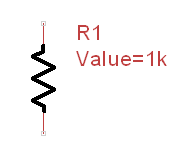
\includegraphics[width=0.15\textwidth]{./pics/SpiceEl/Resistor.png}
  \end{center}
	%\caption{Resistor symbol}
\end{figure}

\textbf{\textit{Schematics Editor Option:}}

"\textsf{Value}" is for assigning an alphanumeric number to \texttt{[VAL]}

\textbf{\textit{Examples:}}

\begin{longtable}{l l}
\textit{statement} & \textit{explanation} \\ \hline \\ \vspace{-0.8\parskip} 
\begin{minipage}{15em}\texttt{r1 1 0 1K}\end{minipage}  
& 
\begin{minipage}{15em}{\small Insert resistor r1, with resistance 1K$\Omega$, between nets 1 and 0}\end{minipage}  \\ \\ 
\begin{minipage}{15em}\texttt{r1 1 0 1K m=2 scale=3}\end{minipage}  
& 
\begin{minipage}{15em}{\small Insert resistor r1, with resistance 1K$\Omega \times \frac{3}{2}$, between nets 1 and 0}\end{minipage} 
\end{longtable}

\textbf{\textit{Remarks:}}

"\textsf{Value}" can be set to a model as described next by the alternative syntax. These alternatives can be used by editing the netlist using the netlist editor.
\newline\noindent
{\color{darkgray}
\textbf{\textit{Alternative Syntax 1:}}

\spicesyntax{\begin{tabular}{l}
RXX [N+] [N-] [VAL] [MODEL] [INLINE PARAMS] \\
.MODEL [MODEL] R [MODEL PARAMS]
\end{tabular}
}

\begin{longtable}{l l}
\textit{parameter} & \textit{description} \\ \hline \\ \vspace{-0.8\parskip}
\texttt{[N+]} & Positive node/net \\
\texttt{[N-]} & Negative node/net \\
\texttt{[VAL]} & Resistance \\
\texttt{[MODEL]} & Resistor model defined by a .model statement \\
\texttt{[INLINE PARAMS]} & \begin{tabular}{lp{5.5cm}p{5cm}}\textit{Inline parameters :} \\ 
																					{\small m : Current multiplication factor} \\ 
																					{\small ac : AC value} \\
																					{\small scale : Current scale factor} \\
																					{\small temp :  Temperature} \\
																					{\small dtemp : Temperature difference with ambient} \\
																					{\small tc1 : Linear temperature coefficient} \\
																					{\small tc2 : Quadratic temperature coefficient} \\
																					{\small noisy : Noise on/off}\end{tabular} \\
\texttt{[MODEL PARAMS]} & \begin{tabular}{lp{5.5cm}p{5cm}}\textit{Model parameters :} \\ 
																					{\small m : Current multiplication factor} \\ 
																					{\small ac : AC value} \\
																					{\small scale : Current scale factor} \\
																					{\small temp :  Temperature} \\
																					{\small dtemp : Temperature difference with ambient} \\
																					{\small tc1 : Linear temperature coefficient} \\
																					{\small tc2 : Quadratic temperature coefficient} \\
																					{\small noisy : Noise on/off}\end{tabular}																					
\end{longtable}

\textbf{\textit{Example:}}

\begin{longtable}{l l}
\textit{statement} & \textit{explanation} \\ \hline \\ %\vspace{-0.1\parskip} 
			\begin{minipage}{15em}{\texttt{r1 1 0 1K res tc1=0.01}\\ 
			\texttt{.model res R m=2}}\end{minipage}
			& \begin{minipage}{15em}{{\small Insert resistor r1, with resistance 1K$\Omega \times \frac{1}{2}$, between nets 1 and 0}}\end{minipage} 
\end{longtable}

\inserttip{If it is specified for an instance, [INLINE PARAMS] override [MODEL PARAMS].} 

\textbf{\textit{Alternative Syntax 2: Semiconductor resistor}}

\spicesyntax{\begin{tabular}{l}
RXX [N+] [N-] [VAL] [MODEL] [INLINE PARAMS] \\
.MODEL [MODEL] R [MODEL PARAMS]
\end{tabular}
}

\begin{longtable}{l l}
\textit{parameter} & \textit{description} \\ \hline \\ \vspace{-0.8\parskip}
\texttt{[N+]} & Positive node/net \\
\texttt{[N-]} & Negative node/net \\
\texttt{[VAL]} & Resistance \\
\texttt{[MODEL]} & Resistor model defined by a .model statement \\
\texttt{[INLINE PARAMS]} & \begin{tabular}{lp{5.5cm}p{5cm}}\textit{Inline parameters :} \\ 
																					{\small l : Length} \\
																					{\small w : Width} \\
																					{\small m : Current multiplication factor} \\ 
																					{\small ac : AC value} \\
																					{\small scale : Current scale factor} \\
																					{\small temp :  Temperature} \\
																					{\small dtemp : Temperature difference with ambient} \\
																					{\small noisy : Noise on/off}\end{tabular} \\
\texttt{[MODEL PARAMS]} & \begin{tabular}{lp{5.5cm}p{5cm}}\textit{Model parameters :} \\ 
																					{\small tc1 : Linear temperature coefficient} \\
																					{\small tc2 : Quadratic temperature coefficient} \\
																					{\small rsh : Sheet resistance} \\
																					{\small defw : Default width} \\
																					{\small narrow : Width narrowing value} \\
																					{\small short : Length shortening value} \\
																					{\small tnom : Nominal temperature} \\
																					{\small kf : Flicker noise coefficient} \\
																					{\small af : Flicker noise exponent} \\
																					{\small r (res) : Default value} \\
																					\end{tabular}																			
\end{longtable}

\textbf{\textit{Example:}}

\begin{longtable}{l l}
\textit{statement} & \textit{explanation} \\ \hline \\ %\vspace{-0.8\parskip} 
		\begin{minipage}{15em}{\texttt{r1 1 0 res l=2u w=1u} \\
			\texttt{.model res R (rsh=10\\+narrow=0.1u short=0.05u)}}\end{minipage} 
			& \begin{minipage}{15em}{{\small Insert resistor r1, with resistance 10$\times\frac{2u-0.05u}{1u-0.1u}\Omega$, between nets 1 and 0}}\end{minipage} 
\end{longtable}

\inserttip{If [VAL] is specified, it will override resistance calculated using the geometrical effects.} 

\textbf{\textit{Remarks:}}

If resistance is not specified, but tc1 (default : 0), tc2 (default : 0), rsh (no default), short (default : 0), and narrow (default : 0) are specified, the semiconductor resistance is calculated using the circuit temperature T as follows:

\begin{eqnarray}
\rm{r} &=& \rm{r}_o\times(1+\rm{tc1}\times(\rm{T}-\rm{tnom})+\rm{tc2}\times(\rm{T}-\rm{tnom})^2) \nonumber\\
\rm{r}_o &=& \rm{rsh}\times\frac{\rm{l}-\rm{short}}{\rm{w}-\rm{narrow}}\nonumber
\end{eqnarray} 

\inserttip{If rsh or l are not specified, r is set to 1m$\Omega$.} 

\textbf{\textit{Alternative Syntax 3: Behavioral resistor}}

\spicesyntax{\begin{tabular}{ll}
RXX & [N+] [N-] R= [EXPRESSION] [INLINE PARAMS]
\end{tabular}
}

\begin{longtable}{l l}
\textit{parameter} & \textit{description} \\ \hline \\ \vspace{-0.8\parskip}
\texttt{[N+]} & Positive node/net \\
\texttt{[N-]} & Negative node/net \\
\texttt{[EXPRESSION]} & An equation or expression containing voltages or currents \\
\texttt{[INLINE PARAMS]} & \begin{tabular}{lp{5.5cm}p{5cm}}\textit{Inline parameters :} \\ 
																					{\small tc1 : Linear temperature coefficient} \\
																					{\small tc2 : Quadratic temperature coefficient} 
																					\end{tabular} 																	
\end{longtable}

\textbf{\textit{Example:}}

\begin{longtable}{l l}
\textit{statement} & \textit{explanation} \\ \hline \\ %\vspace{-0.8\parskip} 
		\begin{minipage}{15em}\texttt{r1 1 0 r={v(2)*0.1}}\end{minipage} 
			& \begin{minipage}{15em}{\small Insert resistor r1, with resistance v(2)$\times$0.1$\Omega$, between nets 1 and 0}\end{minipage} 
\end{longtable}
}

\inserttip{Expression needs to be enclosed with $\{...\}$ or '...'.} 

% CAPACITOR CAPACITOR
\newpage
\subsection{CXX : Capacitors}
\label{subsec_sceadm_capacitors}

\textbf{\textit{Syntax:}}

\spicesyntax{\begin{tabular}{ll}
CXX & [N+] [N-] [VAL] [INLINE PARAMS]
\end{tabular}
}

\begin{longtable}{l l}
\textit{parameter} & \textit{description} \\ \hline \\ \vspace{-0.8\parskip}
\texttt{[N+]} & Positive node/net \\
\texttt{[N-]} & Negative node/net \\
\texttt{[VAL]} & Capacitance \\
\texttt{[INLINE PARAMS]} & \begin{tabular}{lp{5.5cm}p{5cm}}\textit{Inline parameters :}\\ 
																					{\small m : Current multiplication factor} \\ 
																					{\small scale : Current scale factor} \\
																					{\small temp :  Temperature} \\
																					{\small dtemp : Temperature difference with ambient} \\
																					{\small tc1 : Linear temperature coefficient} \\
																					{\small tc2 : Quadratic temperature coefficient} \\
																					{\small ic : Initial condition} \\
																					{\small rser : Series resistance} \\
																					{\small lser : Series inductance} \\ 
																					{\small rpar : Parallel resistance} \\
																					{\small cpar : Parallel capacitance} \\
																					{\small rlshunt : Parallel resistance to lser} 
																					\end{tabular} 
\end{longtable}

\inserttip{rser, lser, rpar, cpar and rlshunt are incorporated for Ltspice compatibility.}

\textbf{\textit{Schematics Editor Library:}}

Analog

\textbf{\textit{Schematics Editor Symbol:}}

\begin{figure}[htb]
  \begin{center}
    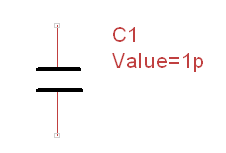
\includegraphics[width=0.15\textwidth]{./pics/SpiceEl/Capacitor.png}
  \end{center}
	%\caption{Resistor symbol}
\end{figure}

\textbf{\textit{Schematics Editor Option:}}

"\textsf{Value}" is for assigning an alphanumeric number to \texttt{[VAL]}

\textbf{\textit{Examples:}}

\begin{longtable}{l l}
\textit{statement} & \textit{explanation} \\ \hline \\ \vspace{-0.8\parskip} 
\begin{minipage}{15em}\texttt{c1 1 0 1p}\end{minipage} & 
\begin{minipage}{15em}{\small Insert capacitor c1, with capacitance 1pF, between nets 1 and 0}\end{minipage} \\
\begin{minipage}{15em}\texttt{c1 1 0 1K m=2 scale=3}\end{minipage} & 
\begin{minipage}{15em}{\small Insert capacitor c1, with capacitance 1pF $\times$2$\times$3, between nets 1 and 0}\end{minipage}
\end{longtable}

\textbf{\textit{Remarks:}}

"\textsf{Value}" can be set to a model as described next by the alternative syntax. These alternatives can be used by editing the netlist using the netlist editor.

\mymarginnote{Default gmin\\is 1e-12} 

\inserttip{CoolSPICE automatically inserts a resistor with resistance 1/gmin across each capacitor to increase stability.}




{\color{darkgray}
\textbf{\textit{Alternative Syntax 1:}}

\spicesyntax{\begin{tabular}{l}
CXX [N+] [N-] [VAL] [MODEL] [INLINE PARAMS] \\
.MODEL [MODEL] C [MODEL PARAMS]
\end{tabular}
}

\begin{longtable}{l l}
\textit{parameter} & \textit{description} \\ \hline \\ \vspace{-0.8\parskip}
\texttt{[N+]} & Positive node/net \\
\texttt{[N-]} & Negative node/net \\
\texttt{[VAL]} & Capacitance \\
\texttt{[MODEL]} & Capacitance model defined by a .model statement \\
\texttt{[INLINE PARAMS]} & \begin{tabular}{lp{5.5cm}p{5cm}}\textit{Inline parameters :} \\ 
																					{\small m : Current multiplication factor} \\ 
																					{\small scale : Current scale factor} \\
																					{\small temp :  Temperature} \\
																					{\small dtemp : Temperature difference with ambient} \\
																					{\small tc1 : Linear temperature coefficient} \\
																					{\small tc2 : Quadratic temperature coefficient} \\
																					{\small ic : Initial condition} \\
																					{\small rser : Series resistance} \\
																					{\small lser : Series inductance} \\ 
																					{\small rpar : Parallel resistance} \\
																					{\small cpar : Parallel capacitance} \\
																					{\small rlshunt : Parallel resistance to lser}																					\end{tabular} \\
\texttt{[MODEL PARAMS]} & \begin{tabular}{lp{5.5cm}p{5cm}}\textit{Model parameters :} \\ 
																					{\small cap : Capacitance} \\
																					{\small m : Current multiplication factor} \\ 
																					{\small scale : Current scale factor} \\
																					{\small temp :  Temperature} \\
																					{\small dtemp : Temperature difference with ambient} \\
																					{\small tc1 : Linear temperature coefficient} \\
																					{\small tc2 : Quadratic temperature coefficient} \\
																					{\small ic : Initial condition}\end{tabular}																					
\end{longtable}

\textbf{\textit{Example:}}

\begin{longtable}{l l}
\textit{statement} & \textit{explanation} \\ \hline \\ %\vspace{-0.1\parskip} 
			\begin{minipage}{15em}{\texttt{c1 1 0 1p cap tc1=0.01}\\ 
			\texttt{.model cap C m=2}}\end{minipage}
			& \begin{minipage}{15em}{{\small Insert capacitor c1, with capacitance 1pF $\times$2, between nets 1 and 0}}\end{minipage} 
\end{longtable}

\inserttip{.ic applies only if uic is used in conjunction with .tran.} 

\textbf{\textit{Alternative Syntax 2: Semiconductor capacitor}}

\spicesyntax{\begin{tabular}{l}
CXX [N+] [N-] [VAL] [MODEL] [INLINE PARAMS] \\
.MODEL [MODEL] C [MODEL PARAMS]
\end{tabular}
}

\begin{longtable}{l l}
\textit{parameter} & \textit{description} \\ \hline \\ \vspace{-0.8\parskip}
\texttt{[N+]} & Positive node/net \\
\texttt{[N-]} & Negative node/net \\
\texttt{[VAL]} & Capacitance \\
\texttt{[MODEL]} & Resistor model defined by a .model statement \\
\texttt{[INLINE PARAMS]} & \begin{tabular}{lp{5.5cm}p{5cm}}\textit{Inline parameters :} \\ 
																					{\small l : Length} \\
																					{\small w : Width} \\
																					{\small m : Current multiplication factor} \\ 
																					{\small scale : Current scale factor} \\
																					{\small temp :  Temperature} \\
																					{\small dtemp : Temperature difference with ambient} \\
																					{\small ic : Initial condition} \\
																					{\small rser : Series resistance} \\
																					{\small lser : Series inductance} \\ 
																					{\small rpar : Parallel resistance} \\
																					{\small cpar : Parallel capacitance} \\
																					{\small rlshunt : Parallel resistance to lser}
																					\end{tabular} \\
\texttt{[MODEL PARAMS]} & \begin{tabular}{lp{5.5cm}p{5cm}}\textit{Model parameters :} \\ 
																					{\small cap : Default value}  \\
																					{\small cj : Bottom/areal junction capacitance} \\
																					{\small cjsw : Sidewall/perimeter junction capacitance} \\
																					{\small defw : Default width} \\
																					{\small defl : Default length} \\
																					{\small defw : Default width} \\
																					{\small narrow : Width narrowing value} \\
																					{\small short : Length shortening value} \\
																					{\small tc1 : Linear temperature coefficient} \\
																					{\small tc2 : Quadratic temperature coefficient} \\
																					{\small tnom : Nominal temperature} \\
																					{\small di : Relative epsilon} \\
																					{\small thick : Dielectric thickness} \\
																					\end{tabular}																			
\end{longtable}

\textbf{\textit{Example:}}

\begin{longtable}{l l}
\textit{statement} & \textit{explanation} \\ \hline \\ %\vspace{-0.8\parskip} 
		\begin{minipage}{15em}{\texttt{c1 1 0 cap l=2u w=1u} \\
			\texttt{.model cap C (cj=1u cjsw=1p)}}\end{minipage} 
			& \begin{minipage}{15em}{{\small Insert capacitor c1, with capacitance 
			1uF/m$^{2}\times\rm{l}\times\rm{w}$ + 1pF/m $\times{2}\times\rm{l}\times\rm{w}$, between nets 1 and 0}}\end{minipage}  
\end{longtable}

\textbf{\textit{Remarks:}}

If cap is not specified, but tc1 (default : 0), tc2 (default : 0), thick (default : 0), short (default : 0), narrow (default : 0), and di (default : 3.9) are specified, the semiconductor capacitance is calculated using the circuit temperature T as follows:

\begin{eqnarray}
\rm{c} &=& \rm{c}_o\times(1+\rm{tc1}\times(\rm{T}-\rm{tnom})+\rm{tc2}\times(\rm{T}-\rm{tnom})^2) \nonumber\\
\rm{c}_o &=& \rm{cj}\times(\rm{l}-\rm{short}) + 2\times\rm{cjsw}\times(\rm{l}-\rm{short}+\rm{w}-\rm{narrow}) \nonumber\\
\rm{cj} &=& \frac{\rm{cj}\times\epsilon_o}{\rm{thick}}\nonumber
\end{eqnarray} 

\inserttip{If [VAL] is specified, it will override capacitance calculated using the geometrical effects.} 

\textbf{\textit{Alternative Syntax 3: Behavioral capacitor}}

\spicesyntax{\begin{tabular}{ll}
CXX & [N+] [N-] C= [EXPRESSION] [INLINE PARAMS]  
\end{tabular}
}

\begin{longtable}{l l}
\textit{parameter} & \textit{description} \\ \hline \\ \vspace{-0.8\parskip}
\texttt{[N+]} & Positive node/net \\
\texttt{[N-]} & Negative node/net \\
\texttt{[EXPRESSION]} & An equation or expression containing voltages or currents \\
\texttt{[INLINE PARAMS]} & \begin{tabular}{lp{5.5cm}p{5cm}}\textit{Inline parameters :} \\ 
																					{\small tc1 : Linear temperature coefficient} \\
																					{\small tc2 : Quadratic temperature coefficient} \\
																					{\small rser : Series resistance} \\
																					{\small lser : Series inductance} \\ 
																					{\small rpar : Parallel resistance} \\
																					{\small cpar : Parallel capacitance} \\
																					{\small rlshunt : Parallel resistance to lser}
																					\end{tabular}  																	
\end{longtable}

\textbf{\textit{Example:}}

\begin{longtable}{l l}
\textit{statement} & \textit{explanation} \\ \hline \\ %\vspace{-0.8\parskip} 
		\begin{minipage}{15em}\texttt{c1 1 0 c={v(2)*0.1}}\end{minipage} 
			& \begin{minipage}{15em}{\small Insert capacitor c1, with capacitance v(2)$\times$0.1F, between nets 1 and 0}\end{minipage} 
\end{longtable}
}

% INDUCTOR INDUCTOR
\newpage
\subsection{LXX : Inductors}
\label{subsec_sceadm_inductors}

\textbf{\textit{Syntax:}}

\spicesyntax{\begin{tabular}{ll}
LXX & [N+] [N-] [VAL] [INLINE PARAMS]
\end{tabular}
}

\begin{longtable}{l l}
\textit{parameter} & \textit{description} \\ \hline \\ \vspace{-0.8\parskip}
\texttt{[N+]} & Positive node/net \\
\texttt{[N-]} & Negative node/net \\
\texttt{[VAL]} & Inductance \\
\texttt{[INLINE PARAMS]} & \begin{tabular}{lp{5.5cm}p{5cm}}\textit{Inline parameters :}\\
																					{\small nt : Number of turns} \\ 
																					{\small m : Current multiplication factor} \\ 
																					{\small scale : Current scale factor} \\
																					{\small temp :  Temperature} \\
																					{\small dtemp : Temperature difference with ambient} \\
																					{\small tc1 : Linear temperature coefficient} \\
																					{\small tc2 : Quadratic temperature coefficient} \\
																					{\small ic : Initial condition} \\
																					{\small rser : Series resistance} \\
																					{\small rpar : Parallel resistance} \\
																					{\small cpar : Parallel capacitance} 
																					\end{tabular} 
\end{longtable}

\inserttip{rser, rpar, and cpar are incorporated for Ltspice compatibility.}

\textbf{\textit{Schematics Editor Library:}}

Analog

\textbf{\textit{Schematics Editor Symbol:}}

\begin{figure}[htb]
  \begin{center}
    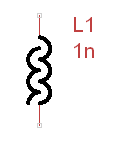
\includegraphics[width=0.125\textwidth]{./pics/SpiceEl/Inductor.png}
  \end{center}
	%\caption{Resistor symbol}
\end{figure}

\textbf{\textit{Schematics Editor Option:}}

"\textsf{Value}" is for assigning an alphanumeric number to \texttt{[VAL]}
\newpage
\textbf{\textit{Examples:}}

\begin{longtable}{l l}
\textit{statement} & \textit{explanation} \\ \hline \\ \vspace{-0.8\parskip} 
\begin{minipage}{15em}\texttt{l1 1 0 1n}\end{minipage} & 
\begin{minipage}{15em}{\small Insert inductor l1, with inductance 1nH, between nets 1 and 0}\end{minipage} \\ \\
\begin{minipage}{15em}\texttt{l1 1 0 1n m=2}\end{minipage} & 
\begin{minipage}{15em}{\small Insert inductor l1, with inductance 1nF $\times$2, between nets 1 and 0}\end{minipage}
\end{longtable}

\textbf{\textit{Remarks:}}

"\textsf{Value}" can be set to a model as described next by the alternative syntax. These alternatives can be used by editing the netlist using the netlist editor.

\mymarginnote{Default gmin\\is 1e-12} 

\inserttip{CoolSPICE automatically inserts a resistor with resistance 1/gmin across each inductor to increase stability.}

\inserttip{CoolSPICE automatically inserts a 1 m$\Omega$ resistor in series with each inductor to increase stability. This can be disabled locally by setting inline parameter 'rser' to zero.}


{\color{darkgray}
\textbf{\textit{Alternative Syntax 1:}}

\spicesyntax{\begin{tabular}{l}
LXX [N+] [N-] [VAL] [MODEL] [INLINE PARAMS] \\
.MODEL [MODEL] L [MODEL PARAMS]
\end{tabular}
}

\begin{longtable}{l l}
\textit{parameter} & \textit{description} \\ \hline \\ \vspace{-0.8\parskip}
\texttt{[N+]} & Positive node/net \\
\texttt{[N-]} & Negative node/net \\
\texttt{[VAL]} & Capacitance \\
\texttt{[MODEL]} & Capacitance model defined by a .model statement \\
\texttt{[INLINE PARAMS]} & \begin{tabular}{lp{5.5cm}p{5cm}}\textit{Inline parameters :} \\ 
																					{\small m : Current multiplication factor} \\ 
																					{\small scale : Current scale factor} \\
																					{\small nt : Number of turns} \\
																					{\small temp :  Temperature} \\
																					{\small dtemp : Temperature difference with ambient} \\
																					{\small tc1 : Linear temperature coefficient} \\
																					{\small tc2 : Quadratic temperature coefficient} \\
																					{\small ic : Initial condition} \\
																					{\small rser : Series resistance} \\
																					{\small rpar : Parallel resistance} \\
																					{\small cpar : Parallel capacitance} 																					\end{tabular} \\
\texttt{[MODEL PARAMS]} & \begin{tabular}{lp{5.5cm}p{5cm}}\textit{Model parameters :} \\ 
																					{\small ind : Capacitance} \\
																					{\small csect : Cross section} \\ 
																					{\small length : Length} \\
																					{\small tc1 : Linear temperature coefficient} \\
																					{\small tc2 : Quadratic temperature coefficient} \\
																					{\small tnom :  Nominal temperature} \\
																					{\small nt : Number of turns} \\
																					{\small mu : Relative $\mu$} \\																					  
																					\end{tabular}																					
\end{longtable}

\textbf{\textit{Example:}}

\begin{longtable}{l l}
\textit{statement} & \textit{explanation} \\ \hline \\ %\vspace{-0.1\parskip} 
			\begin{minipage}{15em}{\texttt{l1 1 0 1n myind tc1=0.01}\\ 
			\texttt{.model myind L m=2}}\end{minipage}
			& \begin{minipage}{15em}
			{{\small Insert inductor l1, with inductance 1nH $\times$0.5, between nets 1 and 0}}
			\end{minipage}
				
\end{longtable}

\inserttip{.ic applies only if uic is used in conjunction with .tran.} 

\textbf{\textit{Remarks:}}

If ind is not specified, but tc1 (default : 0), tc2 (default : 0), nt (default : 0), csect (default : 0), mu (default : 1), and length (default : 0) are specified, the inductance is calculated using the circuit temperature T as follows:

\begin{eqnarray}
\rm{l} &=& \rm{l}_o\times(1+\rm{tc1}\times(\rm{T}-\rm{tnom})+\rm{tc2}\times(\rm{T}-\rm{tnom})^2) \nonumber\\
\rm{l}_o &=& \frac{\rm{mu}\times\mu_o\times\rm{nt}^2\times\rm{csect}}{\rm{length}}\nonumber
\end{eqnarray} 

\inserttip{If [VAL] is specified, it will override inductance calculated using the geometrical effects.} 

\textbf{\textit{Alternative Syntax 3: Behavioral inductor}}

\spicesyntax{\begin{tabular}{ll}
LXX & [N+] [N-] C= [EXPRESSION] [INLINE PARAMS]  
\end{tabular}
}

\begin{longtable}{l l}
\textit{parameter} & \textit{description} \\ \hline \\ \vspace{-0.8\parskip}
\texttt{[N+]} & Positive node/net \\
\texttt{[N-]} & Negative node/net \\
\texttt{[EXPRESSION]} & An equation or expression containing voltages or currents \\
\texttt{[INLINE PARAMS]} & \begin{tabular}{lp{5.5cm}p{5cm}}\textit{Inline parameters :} \\ 
																					{\small tc1 : Linear temperature coefficient} \\
																					{\small tc2 : Quadratic temperature coefficient} \\
																					{\small rser : Series resistance} \\
																					{\small rpar : Parallel resistance} \\
																					{\small cpar : Parallel capacitance} 
																					\end{tabular}  																	
\end{longtable}

\textbf{\textit{Example:}}

\begin{longtable}{l l}
\textit{statement} & \textit{explanation} \\ \hline \\ %\vspace{-0.8\parskip} 
		\begin{minipage}{15em}\texttt{l1 1 0 l={v(2)*0.1}}\end{minipage} 
			& \begin{minipage}{15em}{\small Insert inductor l1, with inductance v(2)$\times$0.1H, between nets 1 and 0}\end{minipage} 
\end{longtable}
}


% COUPLED INDUCTOR COUPLED INDUCTOR
\newpage
\subsection{KXX : Coupled Inductors}
\label{subsec_sceadm_coupledinductors}

\textbf{\textit{Syntax:}}

\spicesyntax{\begin{tabular}{ll}
KXX & [LYY] [LZZ] [VAL] 
\end{tabular}
}

\begin{longtable}{l l}
\textit{parameter} & \textit{description} \\ \hline \\ \vspace{-0.8\parskip}
\texttt{[LYY]} & First of the coupled inductor \\
\texttt{[LZZ]} & Second of the coupled inductor \\
\texttt{[VAL]} & Coupling value \\ 
\end{longtable}

\inserttip{Coupling value has to be between 0 and 1.}

\textbf{\textit{Schematics Editor Library:}}

Analog

\textbf{\textit{Schematics Editor Symbol:}}

\begin{figure}[htb]
  \begin{center}
    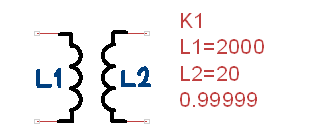
\includegraphics[height=0.08\textheight]{./pics/SpiceEl/CInductor.png}
  \end{center}
	%\caption{Resistor symbol}
\end{figure}

\textbf{\textit{Schematics Editor Option:}}

"\textsf{Value}" is for assigning an alphanumeric number to \texttt{[VAL]}

\textbf{\textit{Examples:}}

\begin{longtable}{l l}
\textit{statement} & \textit{explanation} \\ \hline \\ \vspace{-0.8\parskip} 
\begin{minipage}{15em}\texttt{k1 l1 l2 0.99}\end{minipage} & 
\begin{minipage}{15em}{\small Insert coupled inductor k1, with coupling 0.99, between nets 1 and 0}\end{minipage} \\
\end{longtable}



\newpage
\section{Sources}
\label{sec_sceadm_sources}

\subsection{VXX / IXX :Independent Sources}
\label{subsec_sceadm_independentsources}

\textbf{\textit{Syntax:}}

\spicesyntax{\begin{tabular}{ll}
VXX & [N+] [N-] [DC] [AC] [DISTOF1] [DISTOF2] [FUNCTION]\\
IXX & [N+] [N-] [DC] [AC] [DISTOF1] [DISTOF2] [FUNCTION]
\end{tabular}
}


\begin{longtable}{l l}
\textit{parameter} & \textit{description} \\ \hline \\ \vspace{-0.8\parskip}
\texttt{[N+]} & Positive node/net \\
\texttt{[N-]} & Negative node/net \\
\texttt{[DC]} & DC offset during a DC or transient run \\
\texttt{[AC]} & \begin{tabular}{lp{5.5cm}p{5cm}}\textit{AC parameters :}\\ 
																					{\small ACMAG : AC magnitude} \\ 
																					{\small ACPHASE : AC phase} \\
																					\end{tabular} \\
\texttt{[DISTOF1]} & \begin{tabular}{lp{5.5cm}p{5cm}}\textit{1$^{st}$ distortion parameters :}\\ 
																					{\small F1MAG : Distortion frequency} \\ 
																					{\small F1PHASE : Distortion phase} \\
																					\end{tabular} \\	
\texttt{[DISTOF2]} & \begin{tabular}{lp{5.5cm}p{5cm}}\textit{2$^{nd}$ distortion parameters :}\\ 
																					{\small F2MAG : Distortion frequency} \\ 
																					{\small F2PHASE : Distortion phase} \\
																					\end{tabular} \\
\texttt{[FUNCTION]} & \begin{tabular}{lp{5.5cm}p{5cm}}\textit{Temporal functions :}\\ 
																					{\small Pulse} \\ 
																					{\small Exponential} \\
																					{\small Sinusoidal} \\
																					{\small Piecewise linear} \\
																					{\small Single frequency FM} \\
																					{\small AM} \\
																					{\small Transient noise} \\
																					{\small Random voltages or currents} \\
																					\end{tabular}													
\end{longtable}

\textbf{\textit{Schematics Editor Library:}}

Analog

\textbf{\textit{Schematics Editor Symbol:}}

\begin{figure}[htb]
  \begin{center}
    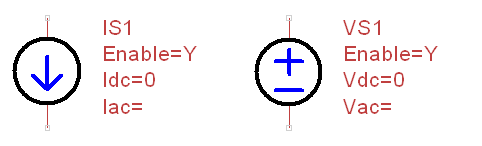
\includegraphics[height=0.08\textheight]{./pics/SpiceEl/IV.png}
  \end{center}
\end{figure}

\textbf{\textit{Schematics Editor Option:}}

"\textsf{Idc / Vdc}"  is for assigning an alphanumeric value to \texttt{[DC]}. "\textsf{Iac / Vac}"  is for assigning an alphanumeric value to \texttt{[AC]}.

\textbf{\textit{Examples:}}

\begin{longtable}{l l}
\textit{statement} & \textit{explanation} \\ \hline \\ \vspace{-0.8\parskip} 
\begin{minipage}{15em}\texttt{v1 1 0 1 0.1}\end{minipage}  
& 
\begin{minipage}{15em}{\small Insert voltage source v1, with 1V DC and 0.1V AC, between nets 1 and 0}\end{minipage}  \\ \\ 
\begin{minipage}{15em}\texttt{i1 1 0 1 0.1}\end{minipage}  
& 
\begin{minipage}{15em}{\small Insert current source i1, with 1V DC and 0.1V AC, between nets 1 and 0}\end{minipage}  \\ \\ 
\begin{minipage}{15em}\texttt{i1 1 0 sin(0 1 1meg)}\end{minipage}  
& 
\begin{minipage}{15em}{\small Insert sinusoidal current source i1, with 1V magnitude and 1MHz frequency, between nets 1 and 0}\end{minipage}
\end{longtable}

\textbf{\textit{Pulse Waveform Syntax:}}

\spicesyntax{\begin{tabular}{l}
PULSE ( [V1] [V2] [TD] [TR] [TF] [PW] [PER] )
\end{tabular}
}

\begin{longtable}{l l}
\textit{parameter} & \textit{description} \\ \hline \\ \vspace{-0.8\parskip}
\texttt{[V1]} & Initial pulse value \\
\texttt{[V2]} & Pulsed value \\
\texttt{[TD]} & Delay time \\
\texttt{[TR]} & Rise time \\
\texttt{[TF]} & Fall time \\
\texttt{[PW]} & Pulse width \\
\texttt{[PER]} & Period
\end{longtable}

\textbf{\textit{Closed Form:}}

  \[
    V(t)=\left\{
                \begin{array}{l l}
                  \rm{V1} \hspace{1.9in} \rm{if\ }0\leq t<\rm{TD}\\
                  \rm{V1}+(\rm{V2}-\rm{V1})\frac{t-\rm{TD}}{\rm{TR}}\hspace{0.55in}\rm{\ if\ TD}\leq t<\rm{TD}+\rm{TR}\\
									\rm{V2} \hspace{1.9in} \rm{if\ TD}+\rm{TR}\leq t<\rm{TD}+\rm{TR}+\rm{PW}\\
                  \rm{V2}+(\rm{V1}-\rm{V2})\frac{t-\rm{TD}-\rm{TR}-\rm{PW}}{\rm{TF}}\rm{\ if\ }\rm{TD}+\rm{TR}+\rm{PW}\leq t<\rm{TD}+\rm{TR}+\rm{PW}+\rm{TF}\\
									\rm{V1} \hspace{1.9in} \rm{if\ }\rm{TD}+\rm{TR}+\rm{PW}+\rm{TF}\leq t<\rm{PER}
                \end{array}
              \right.
  \]

\textbf{\textit{Examples:}}

\begin{longtable}{l l}
\textit{statement} & \textit{explanation} \\ \hline \\ \vspace{-0.8\parskip} 
\begin{minipage}{15em}\texttt{v1 1 0 pulse(0 1 1n 2n 3n 20n 50n)}\end{minipage}  
& 
\begin{minipage}{15em}{\small Insert pulsed voltage source v1 between nets 1 and 0. Pulse source generates a pulse train. The start is delayed by 1ns. The initial DC value is set to the t=0 value. v(1) voltage changes from 0 to 1V between t=1ns and t=3ns. It stays at 1V between t=3ns and t=23ns. It then falls from 1V to 0 between t=23ns and t=26ns. It stays at 0 until t=51ns. 1ns shifted (delayed canceled) version of this initial waveform repeats itself until simulation end time.}\end{minipage}  
\end{longtable}

\textbf{\textit{Sinusoidal Waveform Syntax:}}

\spicesyntax{\begin{tabular}{l}
SIN ( [VO] [VA] [FREQ] [TD] [THETA] )
\end{tabular}
}

\begin{longtable}{l l}
\textit{parameter} & \textit{description} \\ \hline \\ \vspace{-0.8\parskip}
\texttt{[VO]} & Voltage offset \\
\texttt{[VA]} & Sinusoidal wave amplitude \\
\texttt{[FREQ]} & Sinusoidal wave frequency \\
\texttt{[TD]} & Delay time \\
\texttt{[THETA]} & Damping factor 
\end{longtable}

\textbf{\textit{Closed Form:}}

  \[
    V(t)=\left\{
                \begin{array}{l l}
                  \rm{VO} \hspace{3.85in} \rm{if\ }0\leq t<\rm{TD}\\
                  \rm{VO}+\rm{VA}\exp(-(t-\rm{TD})\rm{THETA})\sin(2\pi\rm{FREQ}(t-\rm{TD})) \rm{\ if\ TD}\leq t<\rm{TSTOP}\\
                \end{array}
              \right.
  \]

\textbf{\textit{Examples:}}

\begin{longtable}{l l}
\textit{statement} & \textit{explanation} \\ \hline \\ \vspace{-0.8\parskip} 
\begin{minipage}{15em}\texttt{v1 1 0 sin(0 1 1meg 0 0)}\end{minipage}  
& 
\begin{minipage}{15em}{\small Insert sinusoidal voltage source v1 between nets 1 and 0. The initial DC value is set to the t=0 value. v(1) voltage sinusoidally changes from -1V to 1V with 1MHz frequency.}\end{minipage}  
\end{longtable}

\textbf{\textit{Exponential Waveform Syntax:}}

\spicesyntax{\begin{tabular}{l}
EXP ( [V1] [V2] [TD1] [TAU1] [TD2] [TAU2] )
\end{tabular}
}

\begin{longtable}{l l}
\textit{parameter} & \textit{description} \\ \hline \\ \vspace{-0.8\parskip}
\texttt{[V1]} & Initial value \\
\texttt{[V2]} & Pulsed value \\
\texttt{[TD1]} & Rise delay \\
\texttt{[TAU1]} & Rise time constant \\
\texttt{[TD2]} & Fall delay \\
\texttt{[TAU2]} & Fall time constant
\end{longtable}

\textbf{\textit{Closed Form:}}

  \[
    V(t)=\left\{
                \begin{array}{l l}
                  \rm{V1} \hspace{3.8in} \rm{if\ }0\leq t<\rm{TD1}\\
                  \rm{V1}+(\rm{V2}-\rm{V1})(1-e^{-\frac{t-\rm{TD}}{\rm{TAU1}}})\hspace{1.9in}\rm{\ if\ TD1}\leq t<\rm{TD2}\\
									\rm{V1}+(\rm{V2}-\rm{V1})(1-e^{-\frac{t-\rm{TD1}}{\rm{TAU1}}})+(\rm{V1}-\rm{V2})(1-e^{-\frac{t-\rm{TD2}}{\rm{TAU2}}})\rm{\ if\ TD2}\leq t<\rm{TSTOP}
                \end{array}
              \right.
  \]

\textbf{\textit{Examples:}}

\begin{longtable}{l l}
\textit{statement} & \textit{explanation} \\ \hline \\ \vspace{-0.8\parskip} 
\begin{minipage}{15em}\texttt{v1 1 0 exp(0 1 0 6n 20n 6n)}\end{minipage}  
& 
\begin{minipage}{15em}{\small Insert exponential voltage source v1 between nets 1 and 0. The initial DC value is set to the t=0 value.}\end{minipage}  
\end{longtable}

\textbf{\textit{Piecewise Linear Waveform Syntax:}}

\spicesyntax{\begin{tabular}{l}
PWL ( [T1] [V1] [T2] [V2] [T3] [V3] [T4] [V4] ... ) [INLINE PARAMS]
\end{tabular}
}

\begin{longtable}{l l}
\textit{parameter} & \textit{description} \\ \hline \\ \vspace{-0.8\parskip}
\texttt{[V1] [V2] ...} & Voltage points \\
\texttt{[T1] [T2] ...} & Time points \\
\texttt{[INLINE PARAMS]} & \begin{tabular}{lp{5.5cm}p{5cm}}\textit{Inline parameters :}\\ 
																					{\small r : Repeat interval from r to the last [TN]} \\
																					{\small td : Delay}
																					\end{tabular}  
\end{longtable}

\textbf{\textit{FM Waveform Syntax:}}

\spicesyntax{\begin{tabular}{l}
SFFM ( [VO] [VA] [MDI] [FS] )
\end{tabular}
}

\begin{longtable}{l l}
\textit{parameter} & \textit{description} \\ \hline \\ \vspace{-0.8\parskip}
\texttt{[VO]} & Offset \\
\texttt{[VA]} & Amplitude \\
\texttt{[FC]} & Carrier frequency \\
\texttt{[MDI]} & Modulation \\
\texttt{[FS]} & Signal frequency 
\end{longtable}

\textbf{\textit{Closed Form:}}

  \[
    V(t)=\rm{VO}+\rm{VA}\sin(2\pi\rm{FC}t+\rm{MDI\sin(2\pi\rm{FS}t)}) \nonumber
  \]

%\textbf{\textit{AM Waveform Syntax:}}
%
%\spicesyntax{\begin{tabular}{l}
%AM ( [VA] [VO] [MF] [FC] [TD] )
%\end{tabular}
%}
%
%\begin{longtable}{l l}
%\textit{parameter} & \textit{description} \\ \hline \\ \vspace{-0.8\parskip}
%\texttt{[VA]} & Amplitude \\
%\texttt{[VO]} & Offset \\
%\texttt{[MF]} & Modulating frequency \\
%\texttt{[FC]} & Carrier frequency \\
%\texttt{[TD]} & Delay 
%\end{longtable}
%
%\textbf{\textit{Closed Form:}}
%
  %\[
    %V(t)=\rm{VA}(\rm{VO}+\sin(2\pi\rm{MF}t)\sin(2\pi\rm{FC}t)) \nonumber
  %\]
\newpage
\subsection{GXX / EXX / FXX / HXX : Linear Dependent Sources}
\label{subsec_sceadm_lineardependentsources}

\textbf{\textit{GXX : Voltage Controlled Current Source (VCCS):}}

\spicesyntax{\begin{tabular}{l}
GXX [N+] [N-] [NC+] [NC-] [VAL] 
\end{tabular}
}

\begin{longtable}{l l}
\textit{parameter} & \textit{description} \\ \hline \\ \vspace{-0.8\parskip}
\texttt{[N+]} & Positive current node/net \\
\texttt{[N-]} & Negative current node/net \\
\texttt{[NC+]} & Positive controlling voltage node/net \\
\texttt{[NC-]} & Negative controlling voltage node/net \\
\texttt{[VAL]} & Transconductance
\end{longtable}

\textbf{\textit{Closed Form:}}

  \[
    \rm{I}(\rm{N+}\to\rm{N-})= \rm{VAL}\times(\rm{V}(\rm{NC+})-\rm{V}(\rm{NC-}))\nonumber
  \]
\textbf{\textit{Examples:}}

\begin{longtable}{l l}
\textit{statement} & \textit{explanation} \\ \hline \\ \vspace{-0.8\parskip} 
\begin{minipage}{15em}\texttt{g1 1 0 2 0 2}\end{minipage}  
& 
\begin{minipage}{15em}{\small Insert a current source between nets 1 and 0, and set its value to twice the voltage between 2 and 0.}\end{minipage}  
\end{longtable}

\textbf{\textit{EXX : Voltage Controlled Voltage Source (VCVS):}}

\spicesyntax{\begin{tabular}{l}
EXX [N+] [N-] [NC+] [NC-] [VAL] 
\end{tabular}
}

\begin{longtable}{l l}
\textit{parameter} & \textit{description} \\ \hline \\ \vspace{-0.8\parskip}
\texttt{[N+]} & Positive voltage node/net \\
\texttt{[N-]} & Negative voltage node/net \\
\texttt{[NC+]} & Positive controlling voltage node/net \\
\texttt{[NC-]} & Negative controlling voltage node/net \\
\texttt{[VAL]} & Gain
\end{longtable}

\textbf{\textit{Closed Form:}}

  \[
    (\rm{V}(\rm{N+})-\rm{V}(\rm{N-}))= \rm{VAL}\times(\rm{V}(\rm{NC+})-\rm{V}(\rm{NC-}))\nonumber
  \]
\textbf{\textit{Examples:}}

\begin{longtable}{l l}
\textit{statement} & \textit{explanation} \\ \hline \\ \vspace{-0.8\parskip} 
\begin{minipage}{15em}\texttt{e1 1 0 2 0 2}\end{minipage}  
& 
\begin{minipage}{15em}{\small Insert a voltage source between nets 1 and 0, and set its value to twice the voltage between 2 and 0.}\end{minipage}  
\end{longtable}

\textbf{\textit{FXX : Current Controlled Current Source (CCCS):}}

\spicesyntax{\begin{tabular}{l}
FXX [N+] [N-] [VNAM] [VAL] 
\end{tabular}
}

\begin{longtable}{l l}
\textit{parameter} & \textit{description} \\ \hline \\ \vspace{-0.8\parskip}
\texttt{[N+]} & Positive current node/net \\
\texttt{[N-]} & Negative current node/net \\
\texttt{[VNAM]} & Voltage source  whose current is mirrored \\
\texttt{[VAL]} & Gain
\end{longtable}

\textbf{\textit{Closed Form:}}

  \[
    \rm{I}(\rm{N+}\to\rm{N-})= \rm{VAL}\times\rm{I}(\rm{VNAM})\nonumber
  \]
\textbf{\textit{Examples:}}

\begin{longtable}{l l}
\textit{statement} & \textit{explanation} \\ \hline \\ \vspace{-0.8\parskip} 
\begin{minipage}{15em}\texttt{f1 1 0 v1 2}\end{minipage}  
& 
\begin{minipage}{15em}{\small Insert a current source between nets 1 and 0, and set its value to twice the current flowing on v1.}\end{minipage}  
\end{longtable}

\textbf{\textit{HXX : Current Controlled Voltage Source (CCVS):}}

\spicesyntax{\begin{tabular}{l}
HXX [N+] [N-] [VNAM] [VAL] 
\end{tabular}
}

\begin{longtable}{l l}
\textit{parameter} & \textit{description} \\ \hline \\ \vspace{-0.8\parskip}
\texttt{[N+]} & Positive voltage node/net \\
\texttt{[N-]} & Negative voltage node/net \\
\texttt{[VNAM]} & Voltage source  whose current is mirrored \\
\texttt{[VAL]} & Transresistance
\end{longtable}

\textbf{\textit{Closed Form:}}

  \[
    (\rm{V}(\rm{N+})-\rm{V}(\rm{N-}))= \rm{VAL}\times\rm{I}(\rm{VNAM})\nonumber
  \]
\textbf{\textit{Examples:}}

\begin{longtable}{l l}
\textit{statement} & \textit{explanation} \\ \hline \\ \vspace{-0.8\parskip} 
\begin{minipage}{15em}\texttt{h1 1 0 v1 2}\end{minipage}  
& 
\begin{minipage}{15em}{\small Insert a voltage source between nets 1 and 0, and set its value to twice the current flowing on v1.}\end{minipage}  
\end{longtable}

\newpage
\subsection{BXX : Behavioral Sources}
\label{subsec_sceadm_behavioralsources}

\textbf{\textit{Syntax:}}

\spicesyntax{\begin{tabular}{ll}
BXX & [N+] [N-] [(I/V)] = [EXPRESSION] [INLINE PARAMS]
\end{tabular}
}

\begin{longtable}{l l}
\textit{parameter} & \textit{description} \\ \hline \\ \vspace{-0.8\parskip}
\texttt{[N+]} & Positive node/net \\
\texttt{[N-]} & Negative node/net \\
\texttt{[I/V]} & Current/Voltage \\
\texttt{[EXPRESSION]} & Expression describing current/voltage \\
\texttt{[INLINE PARAMS]}& \begin{tabular}{lp{5.5cm}p{5cm}}\textit{Inline parameters :}\\
	{\small temp : Temperature} \\
	{\small dtemp : Temperature difference from ambient} \\
	{\small tc1 : Linear temperature coefficient} \\
	{\small tc2 : Quadratic temperature coefficient} \\
	{\small rpar : Parallel resistance} \\
	\end{tabular}
\end{longtable}

\textbf{\textit{Schematics Editor Library:}}

Analog

\textbf{\textit{Schematics Editor Symbols:}}

\begin{figure}[htb]
  \begin{center}
    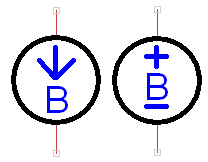
\includegraphics[width=0.15\textwidth]{./pics/SpiceEl/BSource.png}
  \end{center}
\end{figure}

\textbf{\textit{Schematics Editor Option:}}

"\textsf{I/V}" used to describe the current/voltage of the source with an expression \texttt{[I/V]}

\inserttip{One can define the Current OR the voltage of a behavioral source but not both!}

\textbf{\textit{Examples:}}

\begin{longtable}{l l}
%\textit{statement} & \textit{explanation} \\ [0.5ex]
Statement & Explanation \\ [0.5ex]
\hline \\ %\vspace{-0.8\parskip} 

\begin{minipage}{15em}
\texttt{B1 0 1 I=cos(v(1))+sin(v(2))}
\end{minipage}& 
\begin{minipage}{20em}
Insert current source B1, with current equal to the expression cos(v(1))+sin(v(2))
\end{minipage}
\\ \\

\begin{minipage}{15em}
B2 0 1 V=ln(cos(log(v(1,2)\^{}2)))-v(2)\^{}v(1)
\end{minipage} &
\begin{minipage}{20em}
Insert voltage source B2, with voltage equal to the expression V=ln(cos(log(v(1,2)$\rm{^2}$)))-v(2)$\rm{^{v(1)}}$
\end{minipage}
\\ \\

\begin{minipage}{15em}
B3 0 1 V=V(1) $<$ $\left\{\rm{Vlow}\right\}$ ? $\left\{\rm{Vlow}\right\}$ : V(1) $>$ $\left\{\rm{Vhigh}\right\}$ ? $\left\{\rm{Vhigh}\right\}$ : V(1)
\end{minipage} &
\begin{minipage}{20em}
Insert voltage source B3, with voltage equal to the voltage of net/node 1 bounded by parameters 'Vlow' and 'Vhigh'
\end{minipage}
\\ \\

\begin{minipage}{15em}
Bfib 0 1 V=pwl({time}, 0,1, 1,1, 2,2, 3,3, 4,5, 5,8, 6,13, 7,21)
\end{minipage} &
\begin{minipage}{20em}
Insert voltage source Bfib, with voltage equal to the Fibonacci series as a function of time.
\end{minipage}

\end{longtable}

\textbf{\textit{Available functions for behavioral sources:}}

\begin{longtable}{c c}

\hline\hline %inserts double horizontal lines
Function Name & Description \\ [0.5ex] % inserts table
%heading
\hline % inserts single horizontal line
abs(x) & Absolute value of x \\ \\ % inserting body of the table

absdelay(x, del), delay(x, del) & \begin{minipage}{20em}
Value of x del amount of independent units before the current value of the independent variable. If the independent variable is less than the delay parameter del zero.
\end{minipage}\\ \\

arcsin(x), asin(x), arccos(x),\\ 
acos(x), arctan(x), atan(x) & \begin{minipage}{20em}
Inverse trigonometric functions. Note these functions give the real part only.
\end{minipage}\\ \\

asinh(x), acosh(x), atanh(x) & \begin{minipage}{20em}
Inverse hyperbolic trigonometric functions. Note these functions give the real part only.
\end{minipage}\\ \\

atan2(y, x) & \begin{minipage}{20em}
Fourth quadrant inverse tangent of y$/$x
\end{minipage}\\ \\

buf(x) & \begin{minipage}{20em}
(x$>$0.5) ? 1.0 : 0.0
\end{minipage}\\ \\

ceil(x) & \begin{minipage}{20em}
Smallest integer that is greater than or equal to x
\end{minipage}\\ \\

ddt(x) & \begin{minipage}{20em}
derivative of x against the independent variable
\end{minipage}\\ \\

exp(x) & \begin{minipage}{20em}
e$\rm{^x}$
\end{minipage}\\ \\

floor(x), int(x) & \begin{minipage}{20em}
Largest integer that is less than or equal to x
\end{minipage}\\ \\

hypot(x, y) & \begin{minipage}{20em}
sqrt((x$\rm{^2}$) + (y$\rm{^2}$))
\end{minipage}\\ \\

idt(x[,o[,r]]), sdt(x[,o[r]]) & \begin{minipage}{20em}
Integral of x against the independent variable. 'o' is an optional offset parameter. 'r' is an option reset parameter. If 'r' is true the integral resets to 'o'.
\end{minipage}\\ \\

idtmod(x[,ic[,mod[,off]]]), & \begin{minipage}{20em}
Integral of x against the independent variable. 'ic' is an optional initial condition parameter. mod is an optional parameter, the function is reset on reaching mod. 'off' is an optional offset which is added to the output of the function. The effect is to bound the output of the function between zero $+$ offset and 'mod' $+$ offset.
\end{minipage}\\ \\

inv(x) & \begin{minipage}{20em}
(x$>$0.5) ? 0.0 : 1.0
\end{minipage}\\ \\

limit(x, y, z) & \begin{minipage}{20em}
If y $\leq$ x then x, If x $<$ y $<$ z then y, if x $<$ y and z $\leq$ y then z.  
\end{minipage}\\ \\

ln(x), log(x) & \begin{minipage}{20em}
Natural log of absolute value of x, causes error if x is zero
\end{minipage}\\ \\

log10(x) & \begin{minipage}{20em}
Log base ten of absolute value of x, causes error if x is zero
\end{minipage}\\ \\

max(x, y) & \begin{minipage}{20em}
x $>$ y ? x : y
\end{minipage}\\ \\

min(x, y) & \begin{minipage}{20em}
x $<$ y ? x : y
\end{minipage}\\ \\

pow(x, y) & \begin{minipage}{20em}
x raised to the power of y (pow from C runtime library)
\end{minipage}\\ \\

pwr(x, y) & \begin{minipage}{20em}
pow(fabs(x),y), note that this function gives only the real part of the answer
\end{minipage}\\ \\

pwrs(x, y) & \begin{minipage}{20em}
sgn(x)$\cdot$abs(x)$\rm{^y}$
\end{minipage}\\ \\

pwl(x, $\rm{x_1,y_1, x_2,y_2}$...),\\ table(x, $\rm{x_1,y_1, x_2,y_2}$...) & \begin{minipage}{20em}
Piecewise linear function where the answer value y, is interpolated base on the pair of points between which x falls. Note that the x values of the points must increase monotonically.
\end{minipage}\\ \\

rand(x), random(x) & \begin{minipage}{20em}
Randomly generated real number y such that \\0 $<$ y $<$ 1 depending on the integer value of x
\end{minipage}\\ \\

round(x) & \begin{minipage}{20em}
Round to nearest integer, x.5 rounds up.
\end{minipage}\\ \\

sgn(x) & \begin{minipage}{20em}
1.0 for x $>$ 0, 0.0 for x equal to 0, -1.0 for x $<$ 0 
\end{minipage}\\ \\

sin(x), cos(x), tan(x) & \begin{minipage}{20em}
Trigonometric functions
\end{minipage}\\ \\

sinh(x), cosh(x), tanh(x) & \begin{minipage}{20em}
Hyperbolic trigonometric functions
\end{minipage}\\ \\

sqrt(x) & \begin{minipage}{20em}
y=$\sqrt{\rm{x}}$, note that if x is less than zero this function returns the square root of the absolute value of x
\end{minipage}\\ \\

ternary\_fcn(x, y, z), \\
if(x, y, z), x ? y : z & \begin{minipage}{20em}
x ? y : z, (read as "if x then y else z") note the question mark must be followed by a blank space for the parser
\end{minipage}\\ \\

u(x) & \begin{minipage}{20em}
Unit step, x $>$ 0 ? 1 : 0
\end{minipage}\\ \\

unif(nom, rvar) & \begin{minipage}{20em}
Nominal value plus relative variation (to nominal) uniformly distributed between $\pm$rvar
\end{minipage}\\ \\

uramp(x) & \begin{minipage}{20em}
x $>$ 0 ? x : 0
\end{minipage}\\ \\

white(x) & \begin{minipage}{20em}
Randomly generated number y such that -0.5 $<$ y $<$ 0.5
\end{minipage}\\ \\[1ex] % [1ex] adds vertical space
\hline %inserts single line

\caption{Behavioral source functions}
\label {tab:paramfuncs}
\end{longtable}

\textbf{\textit{Available logical operators for behavioral sources: $!=, <>, >=, <=, ==, >, <, ||, \&\&, !$ }}

\subsection{Special Behavioral Source Variables time, temper, temp, hertz}
\textbf{\textit{'time', 'temper' and 'temp' are available in transient for the simulation time and temperature. For example "B1 1 0 v=sin($\rm{\left\{time\right\}}$)" produces a sinusoidal voltage source. 'hertz' is available in AC analyses but may slow the simulation.}}

\newpage
\section{Active Elements}
\label{sec_sceadm_activeelements}

\subsection{DXX : Diodes}
\label{subsec_sceadm_diodes}

\textbf{\textit{Syntax :}}

\spicesyntax{\begin{tabular}{l}
DXX [N+] [N-] [MODEL] [INLINE PARAMS] \\
.MODEL [MODEL] D [MODEL PARAMS]
\end{tabular}
}

\begin{longtable}{l l}
\textit{parameter} & \textit{description} \\ \hline \\ \vspace{-0.8\parskip}
\texttt{[N+]} & Positive node/net \\
\texttt{[N-]} & Negative node/net \\
\texttt{[MODEL]} & Diode model defined by a .model statement \\
\texttt{[INLINE PARAMS]} & \begin{tabular}{lp{5.5cm}p{5cm}}\textit{Inline parameters :} \\ 
																					{\small m : Current multiplication factor} \\ 
																					{\small pj : Perimeter scale factor} \\
																					{\small off : Initial condition for diode state} \\
																					{\small ic :  Initial condition} \\
																					{\small temp : Temperature} \\
																					{\small dtemp : Temperature difference with ambient} \\
																					\end{tabular} 
\end{longtable}

\begin{longtable}{l l}		
\texttt{[MODEL PARAMS]} & \textit{description of model parameters :} \\ \hline \\ \vspace{-0.8\parskip}
																					{\small is} & {\small Saturation current} \\
																					{\small js} & {\small Saturation current} \\
																					{\small jsw} & {\small Sidewall Saturation current} \\
																					{\small tnom} & {\small Parameter measurement temperature} \\
																					{\small tref} & {\small Parameter measurement temperature} \\
																					{\small rs} & {\small Ohmic resistance} \\
																					{\small trs} & {\small Ohmic resistance 1st order temp. coeff.} \\
																					{\small trs1} & {\small Ohmic resistance 1st order temp. coeff.} \\
																					{\small trs2} & {\small Ohmic resistance 2nd order temp. coeff.} \\
																					{\small n} & {\small Emission Coefficient} \\
																					{\small tt} & {\small Transit Time} \\
																					{\small ttt1} & {\small Transit Time 1st order temp. coeff.} \\
																					{\small ttt2} & {\small Transit Time 2nd order temp. coeff.} \\
																					{\small cjo} & {\small Junction capacitance} \\
																					{\small cj0} & {\small Junction capacitance} \\
																					{\small cj} & {\small Junction capacitance} \\
																					{\small vj} & {\small Junction potential} \\
																					{\small pb} & {\small Junction potential} \\
																					
																					{\small m} & {\small Grading coefficient} \\
																					{\small mj} & {\small Grading coefficient} \\
																					{\small tm1} & {\small Grading coefficient 1st temp. coeff.} \\
																					{\small tm2} & {\small Grading coefficient 2nd temp. coeff.} \\
																					{\small cjp} & {\small Sidewall junction capacitance} \\
																					{\small cjsw} & {\small Sidewall junction capacitance} \\
																					{\small php} & {\small Sidewall junction potential} \\
																					{\small mjsw} & {\small Sidewall Grading coefficient} \\
																					{\small ikf} & {\small Forward Knee current} \\
																					{\small ik} & {\small Forward Knee current} \\
																					{\small ikr} & {\small Reverse Knee current} \\
																					{\small tlev} & {\small Diode temperature equation selector} \\
																					{\small tlevc} & {\small Diode temperature equation selector} \\
																					{\small eg} & {\small Activation energy} \\
																					{\small xti} & {\small Saturation current temperature exp.} \\
																					{\small cta} & {\small Area junction temperature coefficient} \\
																					{\small ctc} & {\small Area junction capacitance temperature coefficient} \\
																					{\small ctp} & {\small Perimeter junction capacitance temperature coefficient} \\
																					{\small kf} & {\small Flicker noise coefficient} \\
																					{\small af} & {\small Flicker noise exponent} \\
																					{\small fc} & {\small Forward bias junction fit parameter} \\
																					{\small fcs} & {\small Forward bias sidewall junction fit parameter} \\
																					{\small bv} & {\small Reverse breakdown voltage} \\
																					{\small ibv} & {\small Current at reverse breakdown voltage} \\
																					{\small tcv} & {\small Reverse breakdown voltage temperature coefficient} \\
																					{\small cond} & {\small Ohmic conductance} 
\end{longtable}																				


\textbf{\textit{Temperature Dependent Terms:}}



\newpage
\subsection{QXX : BJTs}
\label{subsec_sceadm_bjts}

\textbf{\textit{Syntax :}}

\spicesyntax{\begin{tabular}{l}
QXX [NC] [NB] [NE] [MODEL] [INLINE PARAMS] \\
.MODEL [MODEL] [DEVICE TYPE] [MODEL PARAMS]
\end{tabular}
}

\begin{longtable}{l l}
\textit{parameter} & \textit{description} \\ \hline \\ \vspace{-0.8\parskip}
\texttt{[NC]} & Collector node/net \\
\texttt{[NB]} & Base node/net \\
\texttt{[NE]} & Emitter node/net (can be followed by an optional source node [NS]) \\
\texttt{[MODEL]} & Bipolar device model defined by a .model statement \\
\texttt{[INLINE PARAMS]} & \begin{tabular}{lp{5.5cm}p{5cm}}\textit{Inline parameters :} \\ 
																					{\small areaa : Emitter area factor} \\ 
																					{\small areab : Base area factor} \\ 
																					{\small areac : Collector area factor} \\ 
																					{\small m : Current multiplication factor} \\ 
																					{\small off : Initial condition for diode state} \\
																					{\small ic :  Initial voltage condition} \\
																					{\small temp : Temperature} \\
																					{\small dtemp : Temperature difference with ambient} \\
																					\end{tabular} \\
\texttt{[DEVICE TYPE]} & NPN or PNP \\																					
\end{longtable}

\begin{longtable}{l l}		
\texttt{[MODEL PARAMS]} & \textit{description of model parameters :} \\ \hline \\ \vspace{-0.8\parskip}
{\small npn} & {\small NPN type device} \\
{\small pnp} & {\small PNP type device} \\
{\small subs} & {\small Vertical or Lateral device} \\
{\small tnom} & {\small Parameter measurement temperature} \\
{\small tref} & {\small Parameter measurement temperature} \\
{\small is} & {\small Saturation Current} \\
{\small bf} & {\small Ideal forward beta} \\
{\small nf} & {\small Forward emission coefficient} \\
{\small vaf} & {\small Forward Early voltage} \\
{\small va} & {\small Forward Early voltage} \\
{\small ikf} & {\small Forward beta roll-off corner current} \\
{\small ik} & {\small Forward beta roll-off corner current} \\
{\small ise} & {\small B-E leakage saturation current} \\
{\small ne} & {\small B-E leakage emission coefficient} \\
{\small br} & {\small Ideal reverse beta} \\
{\small nr} & {\small Reverse emission coefficient} \\
{\small var} & {\small Reverse Early voltage} \\
{\small vb} & {\small Reverse Early voltage} \\
{\small ikr} & {\small reverse beta roll-off corner current} \\
{\small isc} & {\small B-C leakage saturation current} \\
{\small nc} & {\small B-C leakage emission coefficient} \\
{\small rb} & {\small Zero bias base resistance} \\
{\small irb} & {\small Current for base resistance=(rb+rbm)/2} \\
{\small rbm} & {\small Minimum base resistance} \\
{\small re} & {\small Emitter resistance} \\
{\small rc} & {\small Collector resistance} \\
{\small cje} & {\small Zero bias B-E depletion capacitance} \\
{\small vje} & {\small B-E built in potential} \\
{\small pe} & {\small B-E built in potential} \\
{\small mje} & {\small B-E junction grading coefficient} \\
{\small me} & {\small B-E junction grading coefficient} \\
{\small tf} & {\small Ideal forward transit time} \\
{\small xtf} & {\small Coefficient for bias dependence of TF} \\
{\small vtf} & {\small Voltage giving VBC dependence of TF} \\
{\small itf} & {\small High current dependence of TF} \\
{\small ptf} & {\small Excess phase} \\
{\small cjc} & {\small Zero bias B-C depletion capacitance} \\
{\small vjc} & {\small B-C built in potential} \\
{\small pc} & {\small B-C built in potential} \\
{\small mjc} & {\small B-C junction grading coefficient} \\
{\small mc} & {\small B-C junction grading coefficient} \\
{\small xcjc} & {\small Fraction of B-C cap to internal base} \\
{\small tr} & {\small Ideal reverse transit time} \\
{\small cjs} & {\small Zero bias Substrate capacitance} \\
{\small csub} & {\small Zero bias Substrate capacitance} \\
{\small ccs} & {\small Zero bias Substrate capacitance} \\
{\small vjs} & {\small Substrate junction built in potential} \\
{\small ps} & {\small Substrate junction built in potential} \\
{\small mjs} & {\small Substrate junction grading coefficient} \\
{\small ms} & {\small Substrate junction grading coefficient} \\
{\small xtb} & {\small Forward and reverse beta temp. exp.} \\
{\small eg} & {\small Energy gap for IS temp. dependency} \\
{\small xti} & {\small Temp. exponent for IS} \\
{\small fc} & {\small Forward bias junction fit parameter} \\
{\small kf} & {\small Flicker Noise Coefficient} \\
{\small af} & {\small Flicker Noise Exponent} \\
{\small invearlyvoltf} & {\small Inverse early voltage:forward} \\
{\small invearlyvoltr} & {\small Inverse early voltage:reverse} \\
{\small invrollofff} & {\small Inverse roll off - forward} \\
{\small invrolloffr} & {\small Inverse roll off - reverse} \\
{\small collectorconduct} & {\small Collector conductance} \\
{\small emitterconduct} & {\small Emitter conductance} \\
{\small transtimevbcfact} & {\small Transit time VBC factor} \\
{\small excessphasefactor} & {\small Excess phase fact.} \\
{\small iss} & {\small Substrate Jct. Saturation Current} \\
{\small ns} & {\small Substrate current emission coefficient} \\
{\small tlev} & {\small Temperature equation selector} \\
{\small tlevc} & {\small Temperature equation selector} \\
{\small tbf1} & {\small BF 1. temperature coefficient} \\
{\small tbf2} & {\small BF 2. temperature coefficient} \\
{\small tbr1} & {\small BR 1. temperature coefficient} \\
{\small tbr2} & {\small BR 2. temperature coefficient} \\
{\small tikf1} & {\small IKF 1. temperature coefficient} \\
{\small tikf2} & {\small IKF 2. temperature coefficient} \\
{\small tikr1} & {\small IKR 1. temperature coefficient} \\
{\small tikr2} & {\small IKR 2. temperature coefficient} \\
{\small tirb1} & {\small IRB 1. temperature coefficient} \\
{\small tirb2} & {\small IRB 2. temperature coefficient} \\
{\small tnc1} & {\small NC 1. temperature coefficient} \\
{\small tnc2} & {\small NC 2. temperature coefficient} \\
{\small tne1} & {\small NE 1. temperature coefficient} \\
{\small tne2} & {\small NE 2. temperature coefficient} \\
{\small tnf1} & {\small NF 1. temperature coefficient} \\
{\small tnf2} & {\small NF 2. temperature coefficient} \\
{\small tnr1} & {\small NR 1. temperature coefficient} \\
{\small tnr2} & {\small NR 2. temperature coefficient} \\
{\small trb1} & {\small RB 1. temperature coefficient} \\
{\small trb2} & {\small RB 2. temperature coefficient} \\
{\small trc1} & {\small RC 1. temperature coefficient} \\
{\small trc2} & {\small RC 2. temperature coefficient} \\
{\small tre1} & {\small RE 1. temperature coefficient} \\
{\small tre2} & {\small RE 2. temperature coefficient} \\
{\small trm1} & {\small RBM 1. temperature coefficient} \\
{\small trm2} & {\small RBM 2. temperature coefficient} \\
{\small tvaf1} & {\small VAF 1. temperature coefficient} \\
{\small tvaf2} & {\small VAF 2. temperature coefficient} \\
{\small tvar1} & {\small VAR 1. temperature coefficient} \\
{\small tvar2} & {\small VAR 2. temperature coefficient} \\
{\small ctc} & {\small CJC temperature coefficient} \\
{\small cte} & {\small CJE temperature coefficient} \\
{\small cts} & {\small CJS temperature coefficient} \\
{\small tvjc} & {\small VJC temperature coefficient} \\
{\small tvje} & {\small VJE temperature coefficient} \\
{\small tvjs} & {\small VJS temperature coefficient} \\
{\small titf1} & {\small ITF 1. temperature coefficient} \\ 
{\small titf2} & {\small ITF 2. temperature coefficient} \\ 
{\small ttf1} & {\small TF 1. temperature coefficient} \\ 
{\small ttf2} & {\small TF 2. temperature coefficient} \\ 
{\small ttr1} & {\small TR 1. temperature coefficient} \\ 
{\small ttr2} & {\small TR 2. temperature coefficient} \\ 
{\small tmje1} & {\small MJE 1. temperature coefficient} \\
{\small tmje2} & {\small MJE 2. temperature coefficient} \\
{\small tmjc1} & {\small MJC 1. temperature coefficient} \\
{\small tmjc2} & {\small MJC 2. temperature coefficient} \\
{\small tmjs1} & {\small MJS 1. temperature coefficient} \\
{\small tmjs2} & {\small MJS 2. temperature coefficient} \\
{\small tns1} & {\small NS 1. temperature coefficient} \\
{\small tns2} & {\small NS 2. temperature coefficient} \\
{\small nkf} & {\small NKF High current beta rolloff exponent} 
\end{longtable}																				


\textbf{\textit{Example:}}

\begin{longtable}{l l}
\textit{statement} & \textit{explanation} \\ \hline \\ %\vspace{-0.1\parskip} 
			\begin{minipage}{15em}{\texttt{xx}\\ 
			\texttt{.model xx}}\end{minipage}
			& \begin{minipage}{15em}{{\small xx}}\end{minipage} 
\end{longtable}

\newpage
\subsection{MXX : MOSFETs}
\label{subsec_sceadm_mosfets}

\textbf{\textit{Syntax :}}

\spicesyntax{\begin{tabular}{l}
MXX [ND] [NG] [NS] [NB] [MODEL] [INLINE PARAMS] \\
.MODEL [MODEL] [DEVICE TYPE] [MODEL PARAMS]
\end{tabular}
}

\begin{longtable}{l l}
\textit{parameter} & \textit{description} \\ \hline \\ \vspace{-0.8\parskip}
\texttt{[ND]} & Drain node/net \\
\texttt{[NG]} & Gate node/net \\
\texttt{[NS]} & Source node/net \\
\texttt{[NB]} & Body node/net \\
\texttt{[MODEL]} & MOSFET device model defined by a .model statement \\
\texttt{[INLINE PARAMS]} & \begin{tabular}{lp{5.5cm}p{5cm}}\textit{Inline parameters :} \\ 
																					{\small m : Current multiplication factor} \\ 
																					{\small l : Length}\\
																					{\small w : Width} \\
																					{\small ad : Drain area} \\
																					{\small as : Source area} \\
																					{\small pd : Drain perimeter} \\
																					{\small ps : Source perimeter} \\
																					{\small nrd : Number of drain squares} \\
																					{\small nrs : Number of source squares} \\																					{\small off : Initial condition for diode state} \\
																					{\small ic :  Initial voltage condition} \\
																					{\small temp : Temperature} \\
																					\end{tabular} \\
\texttt{[DEVICE TYPE]} & NMOS or PMOS \\																					
\end{longtable}

\begin{longtable}{l l}		
\texttt{[MODEL PARAMS]} & \textit{description of model parameters :} \\ \hline \\ \vspace{-0.8\parskip}

{\small cvchargemod} & {\small Capacitance Charge model selector} \\
{\small capmod} & {\small Capacitance model selector} \\
{\small diomod} & {\small Diode IV model selector} \\
{\small rdsmod} & {\small Bias-dependent S/D resistance model selector} \\
{\small trnqsmod} & {\small Transient NQS model selector} \\
{\small acnqsmod} & {\small AC NQS model selector} \\
{\small mobmod} & {\small Mobility model selector} \\
{\small rbodymod} & {\small Distributed body R model selector} \\
{\small rgatemod} & {\small Gate R model selector} \\
{\small permod} & {\small Pd and Ps model selector} \\
{\small geomod} & {\small Geometry dependent parasitics model selector} \\
{\small fnoimod} & {\small Flicker noise model selector} \\
{\small tnoimod} & {\small Thermal noise model selector} \\
{\small mtrlmod} & {\small parameter for non-silicon substrate or metal gate selector} \\
{\small igcmod} & {\small Gate-to-channel Ig model selector} \\
{\small igbmod} & {\small Gate-to-body Ig model selector} \\
{\small tempmod} & {\small Temperature model selector} \\
{\small paramchk} & {\small Model parameter checking selector} \\
{\small binunit} & {\small Bin  unit  selector} \\
{\small version} & {\small parameter for model version} \\
{\small eot} & {\small Equivalent gate oxide thickness in meters} \\
{\small vddeot} & {\small Voltage for extraction of Equivalent gate oxide thickness} \\
{\small tempeot} & {\small Temperature for extraction of EOT} \\
{\small leffeot} & {\small Effective length for extraction of EOT} \\
{\small weffeot} & {\small Effective width for extraction of EOT} \\
{\small ados} & {\small Charge centroid parameter} \\
{\small bdos} & {\small Charge centroid parameter} \\
{\small toxe} & {\small Electrical gate oxide thickness in meters} \\
{\small toxp} & {\small Physical gate oxide thickness in meters} \\
{\small toxm} & {\small Gate oxide thickness at which parameters are extracted} \\
{\small toxref} & {\small Target tox value} \\
{\small dtox} & {\small Defined as (toxe - toxp) } \\
{\small epsrox} & {\small Dielectric constant of the gate oxide relative to vacuum} \\
{\small cdsc} & {\small Drain/Source and channel coupling capacitance} \\
{\small cdscb} & {\small Body-bias dependence of cdsc} \\ 
{\small cdscd} & {\small Drain-bias dependence of cdsc} \\ 
{\small cit} & {\small Interface state capacitance} \\
{\small nfactor} & {\small Subthreshold swing Coefficient} \\
{\small xj} & {\small Junction depth in meters} \\
{\small vsat} & {\small Saturation velocity at tnom} \\
{\small at} & {\small Temperature coefficient of vsat} \\
{\small a0} & {\small Non-uniform depletion width effect coefficient.} \\ 
{\small ags} & {\small Gate bias  coefficient of Abulk.} \\ 
{\small a1} & {\small Non-saturation effect coefficient} \\
{\small a2} & {\small Non-saturation effect coefficient} \\
{\small keta} & {\small Body-bias coefficient of non-uniform depletion width effect.} \\
{\small phig} & {\small Work function of gate} \\
{\small epsrgate} & {\small Dielectric constant of gate relative to vacuum} \\
{\small easub} & {\small Electron affinity of substrate} \\
{\small epsrsub} & {\small Dielectric constant of substrate relative to vacuum} \\
{\small ni0sub} & {\small Intrinsic carrier concentration of substrate at 300.15K} \\
{\small bg0sub} & {\small Band-gap of substrate at T=0K} \\
{\small tbgasub} & {\small First parameter of band-gap change due to temperature} \\
{\small tbgbsub} & {\small Second parameter of band-gap change due to temperature} \\
{\small nsub} & {\small Substrate doping concentration} \\
{\small ndep} & {\small Channel doping concentration at the depletion edge} \\
{\small nsd} & {\small S/D doping concentration} \\
{\small phin} & {\small Adjusting parameter for surface potential due to non-uniform vertical doping} \\
{\small ngate} & {\small Poly-gate doping concentration} \\
{\small gamma1} & {\small Vth body coefficient} \\
{\small gamma2} & {\small Vth body coefficient} \\
{\small vbx} & {\small Vth transition body Voltage} \\
{\small vbm} & {\small Maximum body voltage} \\

{\small xt} & {\small Doping depth} \\
{\small k1} & {\small Bulk effect coefficient 1} \\
{\small kt1} & {\small Temperature coefficient of Vth} \\
{\small kt1l} & {\small Temperature coefficient of Vth} \\
{\small kt2} & {\small Body-coefficient of kt1} \\
{\small k2} & {\small Bulk effect coefficient 2} \\
{\small k3} & {\small Narrow width effect coefficient} \\
{\small k3b} & {\small Body effect coefficient of k3} \\
{\small w0} & {\small Narrow width effect parameter} \\
{\small dvtp0} & {\small First parameter for Vth shift due to pocket} \\
{\small dvtp1} & {\small Second parameter for Vth shift due to pocket} \\
{\small lpe0} & {\small Equivalent length of pocket region at zero bias} \\
{\small lpeb} & {\small Equivalent length of pocket region accounting for body bias} \\
{\small dvt0} & {\small Short channel effect coeff. 0} \\
{\small dvt1} & {\small Short channel effect coeff. 1} \\
{\small dvt2} & {\small Short channel effect coeff. 2} \\
{\small dvt0w} & {\small Narrow Width coeff. 0} \\
{\small dvt1w} & {\small Narrow Width effect coeff. 1} \\
{\small dvt2w} & {\small Narrow Width effect coeff. 2} \\
{\small drout} & {\small DIBL coefficient of output resistance} \\
{\small dsub} & {\small DIBL coefficient in the subthreshold region} \\
{\small vth0} & {\small Threshold voltage} \\
{\small vtho} & {\small Threshold voltage} \\
{\small ua} & {\small Linear gate dependence of mobility} \\
{\small ua1} & {\small Temperature coefficient of ua} \\
{\small ub} & {\small Quadratic gate dependence of mobility} \\
{\small ub1} & {\small Temperature coefficient of ub} \\
{\small uc} & {\small Body-bias dependence of mobility} \\
{\small uc1} & {\small Temperature coefficient of uc} \\
{\small ud} & {\small Coulomb scattering factor of mobility} \\
{\small ud1} & {\small Temperature coefficient of ud} \\
{\small up} & {\small Channel length linear factor of mobility} \\
{\small lp} & {\small Channel length exponential factor of mobility} \\
{\small u0} & {\small Low-field mobility at Tnom} \\
{\small eu} & {\small Mobility exponent} \\
{\small ucs} & {\small Colombic scattering exponent} \\
{\small ute} & {\small Temperature coefficient of mobility} \\
{\small ucste} & {\small Temperature coefficient of colombic mobility} \\
{\small voff} & {\small Threshold voltage offset} \\
{\small minv} & {\small Fitting parameter for moderate inversion in Vgsteff} \\
{\small minvcv} & {\small Fitting parameter for moderate inversion in Vgsteffcv} \\
{\small voffl} & {\small Length dependence parameter for Vth offset} \\
{\small voffcvl} & {\small Length dependence parameter for Vth offset in CV} \\
{\small tnom} & {\small Parameter measurement temperature} \\
{\small cgso} & {\small Gate-source overlap capacitance per width} \\
{\small cgdo} & {\small Gate-drain overlap capacitance per width} \\
{\small cgbo} & {\small Gate-bulk overlap capacitance per length} \\
{\small xpart} & {\small Channel charge partitioning} \\
{\small delta} & {\small Effective Vds parameter} \\
{\small rsh} & {\small Source-drain sheet resistance} \\
{\small rdsw} & {\small Source-drain resistance per width} \\    
{\small rdswmin} & {\small Source-drain resistance per width at high Vg} \\
{\small rsw} & {\small Source resistance per width} \\
{\small rdw} & {\small Drain resistance per width} \\
{\small rdwmin} & {\small Drain resistance per width at high Vg} \\
{\small rswmin} & {\small Source resistance per width at high Vg} \\

{\small prwg} & {\small Gate-bias effect on parasitic resistance } \\    
{\small prwb} & {\small Body-effect on parasitic resistance } \\    

{\small prt} & {\small Temperature coefficient of parasitic resistance } \\    
{\small eta0} & {\small Subthreshold region DIBL coefficient} \\
{\small etab} & {\small Subthreshold region DIBL coefficient} \\
{\small pclm} & {\small Channel length modulation Coefficient} \\
{\small pdiblc1} & {\small Drain-induced barrier lowering coefficient} \\   
{\small pdiblc2} & {\small Drain-induced barrier lowering coefficient} \\   
{\small pdiblcb} & {\small Body-effect on drain-induced barrier lowering} \\   
{\small fprout} & {\small Rout degradation coefficient for pocket devices} \\
{\small pdits} & {\small Coefficient for drain-induced Vth shifts} \\
{\small pditsl} & {\small Length dependence of drain-induced Vth shifts} \\
{\small pditsd} & {\small Vds dependence of drain-induced Vth shifts} \\
{\small pscbe1} & {\small Substrate current body-effect coefficient} \\   
{\small pscbe2} & {\small Substrate current body-effect coefficient} \\   
{\small pvag} & {\small Gate dependence of output resistance parameter} \\   

{\small jss} & {\small Bottom source junction reverse saturation current density} \\
{\small jsws} & {\small Isolation edge sidewall source junction reverse saturation current density} \\
{\small jswgs} & {\small Gate edge source junction reverse saturation current density} \\
{\small pbs} & {\small Source junction built-in potential} \\
{\small njs} & {\small Source junction emission coefficient} \\
{\small xtis} & {\small Source junction current temperature exponent} \\
{\small mjs} & {\small Source bottom junction capacitance grading coefficient} \\
{\small pbsws} & {\small Source sidewall junction capacitance built in potential} \\
{\small mjsws} & {\small Source sidewall junction capacitance grading coefficient} \\
{\small pbswgs} & {\small Source (gate side) sidewall junction capacitance built in potential} \\
{\small mjswgs} & {\small Source (gate side) sidewall junction capacitance grading coefficient} \\
{\small cjs} & {\small Source bottom junction capacitance per unit area} \\
{\small cjsws} & {\small Source sidewall junction capacitance per unit periphery} \\
{\small cjswgs} & {\small Source (gate side) sidewall junction capacitance per unit width} \\

{\small jsd} & {\small Bottom drain junction reverse saturation current density} \\
{\small jswd} & {\small Isolation edge sidewall drain junction reverse saturation current density} \\
{\small jswgd} & {\small Gate edge drain junction reverse saturation current density} \\
{\small pbd} & {\small Drain junction built-in potential} \\
{\small njd} & {\small Drain junction emission coefficient} \\
{\small xtid} & {\small Drainjunction current temperature exponent} \\
{\small mjd} & {\small Drain bottom junction capacitance grading coefficient} \\
{\small pbswd} & {\small Drain sidewall junction capacitance built in potential} \\
{\small mjswd} & {\small Drain sidewall junction capacitance grading coefficient} \\
{\small pbswgd} & {\small Drain (gate side) sidewall junction capacitance built in potential} \\
{\small mjswgd} & {\small Drain (gate side) sidewall junction capacitance grading coefficient} \\
{\small cjd} & {\small Drain bottom junction capacitance per unit area} \\
{\small cjswd} & {\small Drain sidewall junction capacitance per unit periphery} \\
{\small cjswgd} & {\small Drain (gate side) sidewall junction capacitance per unit width} \\

{\small vfbcv} & {\small Flat Band Voltage parameter for capmod=0 only} \\
{\small vfb} & {\small Flat Band Voltage} \\
{\small tpb} & {\small Temperature coefficient of pb} \\
{\small tcj} & {\small Temperature coefficient of cj} \\
{\small tpbsw} & {\small Temperature coefficient of pbsw} \\
{\small tcjsw} & {\small Temperature coefficient of cjsw} \\
{\small tpbswg} & {\small Temperature coefficient of pbswg} \\
{\small tcjswg} & {\small Temperature coefficient of cjswg} \\
{\small acde} & {\small Exponential coefficient for finite charge thickness} \\
{\small moin} & {\small Coefficient for gate-bias dependent surface potential} \\
{\small noff} & {\small C-V turn-on/off parameter} \\
{\small voffcv} & {\small C-V lateral-shift parameter} \\
{\small dmcg} & {\small Distance of Mid-Contact to Gate edge} \\
{\small dmci} & {\small Distance of Mid-Contact to Isolation} \\
{\small dmdg} & {\small Distance of Mid-Diffusion to Gate edge} \\
{\small dmcgt} & {\small Distance of Mid-Contact to Gate edge in Test structures} \\
{\small xgw} & {\small Distance from gate contact center to device edge} \\
{\small xgl} & {\small Variation in Ldrawn} \\
{\small rshg} & {\small Gate sheet resistance} \\
{\small ngcon} & {\small Number of gate contacts} \\
{\small xrcrg1} & {\small First fitting parameter the bias-dependent Rg} \\
{\small xrcrg2} & {\small Second fitting parameter the bias-dependent Rg} \\
{\small lambda} & {\small Velocity overshoot parameter} \\
{\small vtl} & {\small Thermal velocity} \\
{\small lc} & {\small back scattering parameter} \\
{\small xn} & {\small back scattering parameter} \\
{\small vfbsdoff} & {\small S/D flatband voltage offset} \\
{\small tvfbsdoff} & {\small Temperature parameter for vfbsdoff} \\
{\small tvoff} & {\small Temperature parameter for voff} \\

{\small lintnoi} & {\small lint offset for noise calculation} \\
{\small lint} & {\small Length reduction parameter} \\
{\small ll} & {\small Length reduction parameter} \\
{\small llc} & {\small Length reduction parameter for CV} \\
{\small lln} & {\small Length reduction parameter} \\
{\small lw} & {\small Length reduction parameter} \\
{\small lwc} & {\small Length reduction parameter for CV} \\
{\small lwn} & {\small Length reduction parameter} \\
{\small lwl} & {\small Length reduction parameter} \\
{\small lwlc} & {\small Length reduction parameter for CV} \\
{\small lmin} & {\small Minimum length for the model} \\
{\small lmax} & {\small Maximum length for the model} \\

{\small wr} & {\small Width dependence of rds} \\
{\small wint} & {\small Width reduction parameter} \\
{\small dwg} & {\small Width reduction parameter} \\
{\small dwb} & {\small Width reduction parameter} \\

{\small wl} & {\small Width reduction parameter} \\
{\small wlc} & {\small Width reduction parameter for CV} \\
{\small wln} & {\small Width reduction parameter} \\
{\small ww} & {\small Width reduction parameter} \\
{\small wwc} & {\small Width reduction parameter for CV} \\
{\small wwn} & {\small Width reduction parameter} \\
{\small wwl} & {\small Width reduction parameter} \\
{\small wwlc} & {\small Width reduction parameter for CV} \\
{\small wmin} & {\small Minimum width for the model} \\
{\small wmax} & {\small Maximum width for the model} \\

{\small b0} & {\small Abulk narrow width parameter} \\
{\small b1} & {\small Abulk narrow width parameter} \\

{\small cgsl} & {\small New C-V model parameter} \\
{\small cgdl} & {\small New C-V model parameter} \\
{\small ckappas} & {\small S/G overlap C-V parameter } \\
{\small ckappad} & {\small D/G overlap C-V parameter} \\
{\small cf} & {\small Fringe capacitance parameter} \\
{\small clc} & {\small Vdsat parameter for C-V model} \\
{\small cle} & {\small Vdsat parameter for C-V model} \\
{\small dwc} & {\small Delta W for C-V model} \\
{\small dlc} & {\small Delta L for C-V model} \\
{\small xw} & {\small W offset for channel width due to mask/etch effect} \\
{\small xl} & {\small L offset for channel length due to mask/etch effect} \\
{\small dlcig} & {\small Delta L for Ig model} \\
{\small dlcigd} & {\small Delta L for Ig model drain side} \\
{\small dwj} & {\small Delta W for S/D junctions} \\

{\small alpha0} & {\small substrate current model parameter} \\
{\small alpha1} & {\small substrate current model parameter} \\
{\small beta0} & {\small substrate current model parameter} \\

{\small agidl} & {\small Pre-exponential constant for GIDL} \\
{\small bgidl} & {\small Exponential constant for GIDL} \\
{\small cgidl} & {\small Parameter for body-bias dependence of GIDL} \\
{\small egidl} & {\small Fitting parameter for Bandbending} \\
{\small agisl} & {\small Pre-exponential constant for GISL} \\
{\small bgisl} & {\small Exponential constant for GISL} \\
{\small cgisl} & {\small Parameter for body-bias dependence of GISL} \\
{\small egisl} & {\small Fitting parameter for Bandbending} \\
{\small aigc} & {\small Parameter for Igc} \\
{\small bigc} & {\small Parameter for Igc} \\
{\small cigc} & {\small Parameter for Igc} \\
{\small aigsd} & {\small Parameter for Igs,d} \\
{\small bigsd} & {\small Parameter for Igs,d} \\
{\small cigsd} & {\small Parameter for Igs,d} \\
{\small aigs} & {\small Parameter for Igs} \\
{\small bigs} & {\small Parameter for Igs} \\
{\small cigs} & {\small Parameter for Igs} \\
{\small aigd} & {\small Parameter for Igd} \\
{\small bigd} & {\small Parameter for Igd} \\
{\small cigd} & {\small Parameter for Igd} \\
{\small aigbacc} & {\small Parameter for Igb} \\
{\small bigbacc} & {\small Parameter for Igb} \\
{\small cigbacc} & {\small Parameter for Igb} \\
{\small aigbinv} & {\small Parameter for Igb} \\
{\small bigbinv} & {\small Parameter for Igb} \\
{\small cigbinv} & {\small Parameter for Igb} \\
{\small nigc} & {\small Parameter for Igc slope} \\
{\small nigbinv} & {\small Parameter for Igbinv slope} \\
{\small nigbacc} & {\small Parameter for Igbacc slope} \\
{\small ntox} & {\small Exponent for Tox ratio} \\
{\small eigbinv} & {\small Parameter for the Si bandgap for Igbinv} \\
{\small pigcd} & {\small Parameter for Igc partition} \\
{\small poxedge} & {\small Factor for the gate edge Tox} \\

{\small ijthdfwd} & {\small Forward drain diode forward limiting current} \\
{\small ijthsfwd} & {\small Forward source diode forward limiting current} \\
{\small ijthdrev} & {\small Reverse drain diode forward limiting current} \\
{\small ijthsrev} & {\small Reverse source diode forward limiting current} \\
{\small xjbvd} & {\small Fitting parameter for drain diode breakdown current} \\
{\small xjbvs} & {\small Fitting parameter for source diode breakdown current} \\
{\small bvd} & {\small Drain diode breakdown voltage} \\
{\small bvs} & {\small Source diode breakdown voltage} \\

{\small jtss} & {\small Source bottom trap-assisted saturation current density} \\
{\small jtsd} & {\small Drain bottom trap-assisted saturation current density} \\
{\small jtssws} & {\small Source STI sidewall trap-assisted saturation current density} \\
{\small jtsswd} & {\small Drain STI sidewall trap-assisted saturation current density} \\
{\small jtsswgs} & {\small Source gate-edge sidewall trap-assisted saturation current density} \\
{\small jtsswgd} & {\small Drain gate-edge sidewall trap-assisted saturation current density} \\
{\small jtweff} & {\small TAT current width dependance} \\
{\small njts} & {\small Non-ideality factor for bottom junction} \\
{\small njtssw} & {\small Non-ideality factor for STI sidewall junction} \\
{\small njtsswg} & {\small Non-ideality factor for gate-edge sidewall junction} \\
{\small njtsd} & {\small Non-ideality factor for bottom junction drain side} \\
{\small njtsswd} & {\small Non-ideality factor for STI sidewall junction drain side} \\
{\small njtsswgd} & {\small Non-ideality factor for gate-edge sidewall junction drain side} \\
{\small xtss} & {\small Power dependence of JTSS on temperature} \\
{\small xtsd} & {\small Power dependence of JTSD on temperature} \\
{\small xtssws} & {\small Power dependence of JTSSWS on temperature} \\
{\small xtsswd} & {\small Power dependence of JTSSWD on temperature} \\
{\small xtsswgs} & {\small Power dependence of JTSSWGS on temperature} \\
{\small xtsswgd} & {\small Power dependence of JTSSWGD on temperature} \\
{\small tnjts} & {\small Temperature coefficient for NJTS} \\
{\small tnjtssw} & {\small Temperature coefficient for NJTSSW} \\
{\small tnjtsswg} & {\small Temperature coefficient for NJTSSWG} \\
{\small tnjtsd} & {\small Temperature coefficient for NJTSD} \\
{\small tnjtsswd} & {\small Temperature coefficient for NJTSSWD} \\
{\small tnjtsswgd} & {\small Temperature coefficient for NJTSSWGD} \\
{\small vtss} & {\small Source bottom trap-assisted voltage dependent parameter} \\
{\small vtsd} & {\small Drain bottom trap-assisted voltage dependent parameter} \\
{\small vtssws} & {\small Source STI sidewall trap-assisted voltage dependent parameter} \\
{\small vtsswd} & {\small Drain STI sidewall trap-assisted voltage dependent parameter} \\
{\small vtsswgs} & {\small Source gate-edge sidewall trap-assisted voltage dependent parameter} \\
{\small vtsswgd} & {\small Drain gate-edge sidewall trap-assisted voltage dependent parameter} \\

{\small gbmin} & {\small Minimum body conductance} \\
{\small rbdb} & {\small Resistance between bNode and dbNode} \\
{\small rbpb} & {\small Resistance between bNodePrime and bNode} \\
{\small rbsb} & {\small Resistance between bNode and sbNode} \\
{\small rbps} & {\small Resistance between bNodePrime and sbNode} \\
{\small rbpd} & {\small Resistance between bNodePrime and bNode} \\

{\small rbps0} & {\small Body resistance RBPS scaling} \\
{\small rbpsl} & {\small Body resistance RBPS L scaling} \\
{\small rbpsw} & {\small Body resistance RBPS W scaling} \\
{\small rbpsnf} & {\small Body resistance RBPS NF scaling} \\

{\small rbpd0} & {\small Body resistance RBPD scaling} \\
{\small rbpdl} & {\small Body resistance RBPD L scaling} \\
{\small rbpdw} & {\small Body resistance RBPD W scaling} \\
{\small rbpdnf} & {\small Body resistance RBPD NF scaling} \\

{\small rbpbx0} & {\small Body resistance RBPBX  scaling} \\
{\small rbpbxl} & {\small Body resistance RBPBX L scaling} \\
{\small rbpbxw} & {\small Body resistance RBPBX W scaling} \\
{\small rbpbxnf} & {\small Body resistance RBPBX NF scaling} \\
{\small rbpby0} & {\small Body resistance RBPBY  scaling} \\
{\small rbpbyl} & {\small Body resistance RBPBY L scaling} \\
{\small rbpbyw} & {\small Body resistance RBPBY W scaling} \\
{\small rbpbynf} & {\small Body resistance RBPBY NF scaling} \\

{\small rbsbx0} & {\small Body resistance RBSBX  scaling} \\
{\small rbsby0} & {\small Body resistance RBSBY  scaling} \\
{\small rbdbx0} & {\small Body resistance RBDBX  scaling} \\
{\small rbdby0} & {\small Body resistance RBDBY  scaling} \\

{\small rbsdbxl} & {\small Body resistance RBSDBX L scaling} \\
{\small rbsdbxw} & {\small Body resistance RBSDBX W scaling} \\
{\small rbsdbxnf} & {\small Body resistance RBSDBX NF scaling} \\
{\small rbsdbyl} & {\small Body resistance RBSDBY L scaling} \\
{\small rbsdbyw} & {\small Body resistance RBSDBY W scaling} \\
{\small rbsdbynf} & {\small Body resistance RBSDBY NF scaling} \\

{\small lcdsc} & {\small Length dependence of cdsc} \\
{\small lcdscb} & {\small Length dependence of cdscb} \\
{\small lcdscd} & {\small Length dependence of cdscd} \\
{\small lcit} & {\small Length dependence of cit} \\
{\small lnfactor} & {\small Length dependence of nfactor} \\
{\small lxj} & {\small Length dependence of xj} \\
{\small lvsat} & {\small Length dependence of vsat} \\
{\small lat} & {\small Length dependence of at} \\
{\small la0} & {\small Length dependence of a0} \\ 
{\small lags} & {\small Length dependence of ags} \\ 
{\small la1} & {\small Length dependence of a1} \\
{\small la2} & {\small Length dependence of a2} \\
{\small lketa} & {\small Length dependence of keta} \\
{\small lnsub} & {\small Length dependence of nsub} \\
{\small lndep} & {\small Length dependence of ndep} \\
{\small lnsd} & {\small Length dependence of nsd} \\
{\small lphin} & {\small Length dependence of phin} \\
{\small lngate} & {\small Length dependence of ngate} \\
{\small lgamma1} & {\small Length dependence of gamma1} \\
{\small lgamma2} & {\small Length dependence of gamma2} \\
{\small lvbx} & {\small Length dependence of vbx} \\
{\small lvbm} & {\small Length dependence of vbm} \\
{\small lxt} & {\small Length dependence of xt} \\
{\small lk1} & {\small Length dependence of k1} \\
{\small lkt1} & {\small Length dependence of kt1} \\
{\small lkt1l} & {\small Length dependence of kt1l} \\
{\small lkt2} & {\small Length dependence of kt2} \\
{\small lk2} & {\small Length dependence of k2} \\
{\small lk3} & {\small Length dependence of k3} \\
{\small lk3b} & {\small Length dependence of k3b} \\
{\small lw0} & {\small Length dependence of w0} \\
{\small ldvtp0} & {\small Length dependence of dvtp0} \\
{\small ldvtp1} & {\small Length dependence of dvtp1} \\
{\small llpe0} & {\small Length dependence of lpe0} \\
{\small llpeb} & {\small Length dependence of lpeb} \\
{\small ldvt0} & {\small Length dependence of dvt0} \\
{\small ldvt1} & {\small Length dependence of dvt1} \\
{\small ldvt2} & {\small Length dependence of dvt2} \\
{\small ldvt0w} & {\small Length dependence of dvt0w} \\
{\small ldvt1w} & {\small Length dependence of dvt1w} \\
{\small ldvt2w} & {\small Length dependence of dvt2w} \\
{\small ldrout} & {\small Length dependence of drout} \\
{\small ldsub} & {\small Length dependence of dsub} \\
{\small lvth0} & {\small Length dependence of vto} \\
{\small lvtho} & {\small Length dependence of vto} \\
{\small lua} & {\small Length dependence of ua} \\
{\small lua1} & {\small Length dependence of ua1} \\
{\small lub} & {\small Length dependence of ub} \\
{\small lub1} & {\small Length dependence of ub1} \\
{\small luc} & {\small Length dependence of uc} \\
{\small luc1} & {\small Length dependence of uc1} \\
{\small lud} & {\small Length dependence of ud} \\
{\small lud1} & {\small Length dependence of ud1} \\
{\small lup} & {\small Length dependence of up} \\
{\small llp} & {\small Length dependence of lp} \\
{\small lu0} & {\small Length dependence of u0} \\
{\small lute} & {\small Length dependence of ute} \\
{\small lucste} & {\small Length dependence of ucste} \\
{\small lvoff} & {\small Length dependence of voff} \\
{\small lminv} & {\small Length dependence of minv} \\
{\small lminvcv} & {\small Length dependence of minvcv} \\
{\small ldelta} & {\small Length dependence of delta} \\
{\small lrdsw} & {\small Length dependence of rdsw } \\    
{\small lrsw} & {\small Length dependence of rsw} \\
{\small lrdw} & {\small Length dependence of rdw} \\

{\small lprwg} & {\small Length dependence of prwg } \\    
{\small lprwb} & {\small Length dependence of prwb } \\    

{\small lprt} & {\small Length dependence of prt } \\    
{\small leta0} & {\small Length dependence of eta0} \\   
{\small letab} & {\small Length dependence of etab} \\   
{\small lpclm} & {\small Length dependence of pclm} \\   
{\small lpdiblc1} & {\small Length dependence of pdiblc1} \\   
{\small lpdiblc2} & {\small Length dependence of pdiblc2} \\   
{\small lpdiblcb} & {\small Length dependence of pdiblcb} \\   
{\small lfprout} & {\small Length dependence of pdiblcb} \\
{\small lpdits} & {\small Length dependence of pdits} \\
{\small lpditsd} & {\small Length dependence of pditsd} \\
{\small lpscbe1} & {\small Length dependence of pscbe1} \\   
{\small lpscbe2} & {\small Length dependence of pscbe2} \\   
{\small lpvag} & {\small Length dependence of pvag} \\   
{\small lwr} & {\small Length dependence of wr} \\
{\small ldwg} & {\small Length dependence of dwg} \\
{\small ldwb} & {\small Length dependence of dwb} \\
{\small lb0} & {\small Length dependence of b0} \\
{\small lb1} & {\small Length dependence of b1} \\
{\small lcgsl} & {\small Length dependence of cgsl} \\
{\small lcgdl} & {\small Length dependence of cgdl} \\
{\small lckappas} & {\small Length dependence of ckappas} \\
{\small lckappad} & {\small Length dependence of ckappad} \\
{\small lcf} & {\small Length dependence of cf} \\
{\small lclc} & {\small Length dependence of clc} \\
{\small lcle} & {\small Length dependence of cle} \\
{\small lalpha0} & {\small Length dependence of alpha0} \\
{\small lalpha1} & {\small Length dependence of alpha1} \\
{\small lbeta0} & {\small Length dependence of beta0} \\

{\small lagidl} & {\small Length dependence of agidl} \\
{\small lbgidl} & {\small Length dependence of bgidl} \\
{\small lcgidl} & {\small Length dependence of cgidl} \\
{\small legidl} & {\small Length dependence of egidl} \\
{\small lagisl} & {\small Length dependence of agisl} \\
{\small lbgisl} & {\small Length dependence of bgisl} \\
{\small lcgisl} & {\small Length dependence of cgisl} \\
{\small legisl} & {\small Length dependence of egisl} \\
{\small laigc} & {\small Length dependence of aigc} \\
{\small lbigc} & {\small Length dependence of bigc} \\
{\small lcigc} & {\small Length dependence of cigc} \\
{\small laigsd} & {\small Length dependence of aigsd} \\
{\small lbigsd} & {\small Length dependence of bigsd} \\
{\small lcigsd} & {\small Length dependence of cigsd} \\
{\small laigs} & {\small Length dependence of aigs} \\
{\small lbigs} & {\small Length dependence of bigs} \\
{\small lcigs} & {\small Length dependence of cigs} \\
{\small laigd} & {\small Length dependence of aigd} \\
{\small lbigd} & {\small Length dependence of bigd} \\
{\small lcigd} & {\small Length dependence of cigd} \\
{\small laigbacc} & {\small Length dependence of aigbacc} \\
{\small lbigbacc} & {\small Length dependence of bigbacc} \\
{\small lcigbacc} & {\small Length dependence of cigbacc} \\
{\small laigbinv} & {\small Length dependence of aigbinv} \\
{\small lbigbinv} & {\small Length dependence of bigbinv} \\
{\small lcigbinv} & {\small Length dependence of cigbinv} \\
{\small lnigc} & {\small Length dependence of nigc} \\
{\small lnigbinv} & {\small Length dependence of nigbinv} \\
{\small lnigbacc} & {\small Length dependence of nigbacc} \\
{\small lntox} & {\small Length dependence of ntox} \\
{\small leigbinv} & {\small Length dependence for eigbinv} \\
{\small lpigcd} & {\small Length dependence for pigcd} \\
{\small lpoxedge} & {\small Length dependence for poxedge} \\

{\small lvfbcv} & {\small Length dependence of vfbcv} \\
{\small lvfb} & {\small Length dependence of vfb} \\
{\small lacde} & {\small Length dependence of acde} \\
{\small lmoin} & {\small Length dependence of moin} \\
{\small lnoff} & {\small Length dependence of noff} \\
{\small lvoffcv} & {\small Length dependence of voffcv} \\
{\small lxrcrg1} & {\small Length dependence of xrcrg1} \\
{\small lxrcrg2} & {\small Length dependence of xrcrg2} \\
{\small llambda} & {\small Length dependence of lambda} \\
{\small lvtl} & {\small Length dependence of vtl} \\
{\small lxn} & {\small Length dependence of xn} \\
{\small leu} & {\small Length dependence of eu} \\
{\small lucs} & {\small Length dependence of lucs} \\
{\small lvfbsdoff} & {\small Length dependence of vfbsdoff} \\
{\small ltvfbsdoff} & {\small Length dependence of tvfbsdoff} \\
{\small ltvoff} & {\small Length dependence of tvoff} \\

{\small wcdsc} & {\small Width dependence of cdsc} \\
{\small wcdscb} & {\small Width dependence of cdscb} \\  
{\small wcdscd} & {\small Width dependence of cdscd} \\  
{\small wcit} & {\small Width dependence of cit} \\
{\small wnfactor} & {\small Width dependence of nfactor} \\
{\small wxj} & {\small Width dependence of xj} \\
{\small wvsat} & {\small Width dependence of vsat} \\
{\small wat} & {\small Width dependence of at} \\
{\small wa0} & {\small Width dependence of a0} \\ 
{\small wags} & {\small Width dependence of ags} \\ 
{\small wa1} & {\small Width dependence of a1} \\
{\small wa2} & {\small Width dependence of a2} \\
{\small wketa} & {\small Width dependence of keta} \\
{\small wnsub} & {\small Width dependence of nsub} \\
{\small wndep} & {\small Width dependence of ndep} \\
{\small wnsd} & {\small Width dependence of nsd} \\
{\small wphin} & {\small Width dependence of phin} \\
{\small wngate} & {\small Width dependence of ngate} \\
{\small wgamma1} & {\small Width dependence of gamma1} \\
{\small wgamma2} & {\small Width dependence of gamma2} \\
{\small wvbx} & {\small Width dependence of vbx} \\
{\small wvbm} & {\small Width dependence of vbm} \\
{\small wxt} & {\small Width dependence of xt} \\
{\small wk1} & {\small Width dependence of k1} \\
{\small wkt1} & {\small Width dependence of kt1} \\
{\small wkt1l} & {\small Width dependence of kt1l} \\
{\small wkt2} & {\small Width dependence of kt2} \\
{\small wk2} & {\small Width dependence of k2} \\
{\small wk3} & {\small Width dependence of k3} \\
{\small wk3b} & {\small Width dependence of k3b} \\
{\small ww0} & {\small Width dependence of w0} \\
{\small wdvtp0} & {\small Width dependence of dvtp0} \\
{\small wdvtp1} & {\small Width dependence of dvtp1} \\
{\small wlpe0} & {\small Width dependence of lpe0} \\
{\small wlpeb} & {\small Width dependence of lpeb} \\
{\small wdvt0} & {\small Width dependence of dvt0} \\
{\small wdvt1} & {\small Width dependence of dvt1} \\
{\small wdvt2} & {\small Width dependence of dvt2} \\
{\small wdvt0w} & {\small Width dependence of dvt0w} \\
{\small wdvt1w} & {\small Width dependence of dvt1w} \\
{\small wdvt2w} & {\small Width dependence of dvt2w} \\
{\small wdrout} & {\small Width dependence of drout} \\
{\small wdsub} & {\small Width dependence of dsub} \\
{\small wvth0} & {\small Width dependence of vto} \\
{\small wvtho} & {\small Width dependence of vto} \\
{\small wua} & {\small Width dependence of ua} \\
{\small wua1} & {\small Width dependence of ua1} \\
{\small wub} & {\small Width dependence of ub} \\
{\small wub1} & {\small Width dependence of ub1} \\
{\small wuc} & {\small Width dependence of uc} \\
{\small wuc1} & {\small Width dependence of uc1} \\
{\small wud} & {\small Width dependence of ud} \\
{\small wud1} & {\small Width dependence of ud1} \\
{\small wup} & {\small Width dependence of up} \\
{\small wlp} & {\small Width dependence of lp} \\
{\small wu0} & {\small Width dependence of u0} \\
{\small wute} & {\small Width dependence of ute} \\
{\small wucste} & {\small Width dependence of ucste} \\
{\small wvoff} & {\small Width dependence of voff} \\
{\small wminv} & {\small Width dependence of minv} \\
{\small wminvcv} & {\small Width dependence of minvcv} \\
{\small wdelta} & {\small Width dependence of delta} \\
{\small wrdsw} & {\small Width dependence of rdsw } \\
{\small wrsw} & {\small Width dependence of rsw} \\
{\small wrdw} & {\small Width dependence of rdw} \\

{\small wprwg} & {\small Width dependence of prwg } \\
{\small wprwb} & {\small Width dependence of prwb } \\

{\small wprt} & {\small Width dependence of prt} \\
{\small weta0} & {\small Width dependence of eta0} \\   
{\small wetab} & {\small Width dependence of etab} \\   
{\small wpclm} & {\small Width dependence of pclm} \\   
{\small wpdiblc1} & {\small Width dependence of pdiblc1} \\   
{\small wpdiblc2} & {\small Width dependence of pdiblc2} \\   
{\small wpdiblcb} & {\small Width dependence of pdiblcb} \\   
{\small wfprout} & {\small Width dependence of pdiblcb} \\
{\small wpdits} & {\small Width dependence of pdits} \\
{\small wpditsd} & {\small Width dependence of pditsd} \\
{\small wpscbe1} & {\small Width dependence of pscbe1} \\   
{\small wpscbe2} & {\small Width dependence of pscbe2} \\   
{\small wpvag} & {\small Width dependence of pvag} \\   
{\small wwr} & {\small Width dependence of wr} \\
{\small wdwg} & {\small Width dependence of dwg} \\
{\small wdwb} & {\small Width dependence of dwb} \\
{\small wb0} & {\small Width dependence of b0} \\
{\small wb1} & {\small Width dependence of b1} \\
{\small wcgsl} & {\small Width dependence of cgsl} \\
{\small wcgdl} & {\small Width dependence of cgdl} \\
{\small wckappas} & {\small Width dependence of ckappas} \\
{\small wckappad} & {\small Width dependence of ckappad} \\
{\small wcf} & {\small Width dependence of cf} \\
{\small wclc} & {\small Width dependence of clc} \\
{\small wcle} & {\small Width dependence of cle} \\
{\small walpha0} & {\small Width dependence of alpha0} \\
{\small walpha1} & {\small Width dependence of alpha1} \\
{\small wbeta0} & {\small Width dependence of beta0} \\

{\small wagidl} & {\small Width dependence of agidl} \\
{\small wbgidl} & {\small Width dependence of bgidl} \\
{\small wcgidl} & {\small Width dependence of cgidl} \\
{\small wegidl} & {\small Width dependence of egidl} \\
{\small wagisl} & {\small Width dependence of agisl} \\
{\small wbgisl} & {\small Width dependence of bgisl} \\
{\small wcgisl} & {\small Width dependence of cgisl} \\
{\small wegisl} & {\small Width dependence of egisl} \\
{\small waigc} & {\small Width dependence of aigc} \\
{\small wbigc} & {\small Width dependence of bigc} \\
{\small wcigc} & {\small Width dependence of cigc} \\
{\small waigsd} & {\small Width dependence of aigsd} \\
{\small wbigsd} & {\small Width dependence of bigsd} \\
{\small wcigsd} & {\small Width dependence of cigsd} \\
{\small waigs} & {\small Width dependence of aigs} \\
{\small wbigs} & {\small Width dependence of bigs} \\
{\small wcigs} & {\small Width dependence of cigs} \\
{\small waigd} & {\small Width dependence of aigd} \\
{\small wbigd} & {\small Width dependence of bigd} \\
{\small wcigd} & {\small Width dependence of cigd} \\
{\small waigbacc} & {\small Width dependence of aigbacc} \\
{\small wbigbacc} & {\small Width dependence of bigbacc} \\
{\small wcigbacc} & {\small Width dependence of cigbacc} \\
{\small waigbinv} & {\small Width dependence of aigbinv} \\
{\small wbigbinv} & {\small Width dependence of bigbinv} \\
{\small wcigbinv} & {\small Width dependence of cigbinv} \\
{\small wnigc} & {\small Width dependence of nigc} \\
{\small wnigbinv} & {\small Width dependence of nigbinv} \\
{\small wnigbacc} & {\small Width dependence of nigbacc} \\
{\small wntox} & {\small Width dependence of ntox} \\
{\small weigbinv} & {\small Width dependence for eigbinv} \\
{\small wpigcd} & {\small Width dependence for pigcd} \\
{\small wpoxedge} & {\small Width dependence for poxedge} \\
{\small wvfbcv} & {\small Width dependence of vfbcv} \\
{\small wvfb} & {\small Width dependence of vfb} \\
{\small wacde} & {\small Width dependence of acde} \\
{\small wmoin} & {\small Width dependence of moin} \\
{\small wnoff} & {\small Width dependence of noff} \\
{\small wvoffcv} & {\small Width dependence of voffcv} \\
{\small wxrcrg1} & {\small Width dependence of xrcrg1} \\
{\small wxrcrg2} & {\small Width dependence of xrcrg2} \\
{\small wlambda} & {\small Width dependence of lambda} \\
{\small wvtl} & {\small Width dependence of vtl} \\
{\small wxn} & {\small Width dependence of xn} \\
{\small weu} & {\small Width dependence of eu} \\
{\small wucs} & {\small Width dependence of ucs} \\
{\small wvfbsdoff} & {\small Width dependence of vfbsdoff} \\
{\small wtvfbsdoff} & {\small Width dependence of tvfbsdoff} \\
{\small wtvoff} & {\small Width dependence of tvoff} \\

{\small pcdsc} & {\small Cross-term dependence of cdsc} \\
{\small pcdscb} & {\small Cross-term dependence of cdscb} \\ 
{\small pcdscd} & {\small Cross-term dependence of cdscd} \\
{\small pcit} & {\small Cross-term dependence of cit} \\
{\small pnfactor} & {\small Cross-term dependence of nfactor} \\
{\small pxj} & {\small Cross-term dependence of xj} \\
{\small pvsat} & {\small Cross-term dependence of vsat} \\
{\small pat} & {\small Cross-term dependence of at} \\
{\small pa0} & {\small Cross-term dependence of a0} \\ 
{\small pags} & {\small Cross-term dependence of ags} \\
{\small pa1} & {\small Cross-term dependence of a1} \\
{\small pa2} & {\small Cross-term dependence of a2} \\
{\small pketa} & {\small Cross-term dependence of keta} \\
{\small pnsub} & {\small Cross-term dependence of nsub} \\
{\small pndep} & {\small Cross-term dependence of ndep} \\
{\small pnsd} & {\small Cross-term dependence of nsd} \\
{\small pphin} & {\small Cross-term dependence of phin} \\
{\small pngate} & {\small Cross-term dependence of ngate} \\
{\small pgamma1} & {\small Cross-term dependence of gamma1} \\
{\small pgamma2} & {\small Cross-term dependence of gamma2} \\
{\small pvbx} & {\small Cross-term dependence of vbx} \\
{\small pvbm} & {\small Cross-term dependence of vbm} \\
{\small pxt} & {\small Cross-term dependence of xt} \\
{\small pk1} & {\small Cross-term dependence of k1} \\
{\small pkt1} & {\small Cross-term dependence of kt1} \\
{\small pkt1l} & {\small Cross-term dependence of kt1l} \\
{\small pkt2} & {\small Cross-term dependence of kt2} \\
{\small pk2} & {\small Cross-term dependence of k2} \\
{\small pk3} & {\small Cross-term dependence of k3} \\
{\small pk3b} & {\small Cross-term dependence of k3b} \\
{\small pw0} & {\small Cross-term dependence of w0} \\
{\small pdvtp0} & {\small Cross-term dependence of dvtp0} \\
{\small pdvtp1} & {\small Cross-term dependence of dvtp1} \\
{\small plpe0} & {\small Cross-term dependence of lpe0} \\
{\small plpeb} & {\small Cross-term dependence of lpeb} \\
{\small pdvt0} & {\small Cross-term dependence of dvt0} \\
{\small pdvt1} & {\small Cross-term dependence of dvt1} \\
{\small pdvt2} & {\small Cross-term dependence of dvt2} \\
{\small pdvt0w} & {\small Cross-term dependence of dvt0w} \\
{\small pdvt1w} & {\small Cross-term dependence of dvt1w} \\
{\small pdvt2w} & {\small Cross-term dependence of dvt2w} \\
{\small pdrout} & {\small Cross-term dependence of drout} \\
{\small pdsub} & {\small Cross-term dependence of dsub} \\
{\small pvth0} & {\small Cross-term dependence of vto} \\
{\small pvtho} & {\small Cross-term dependence of vto} \\
{\small pua} & {\small Cross-term dependence of ua} \\
{\small pua1} & {\small Cross-term dependence of ua1} \\
{\small pub} & {\small Cross-term dependence of ub} \\
{\small pub1} & {\small Cross-term dependence of ub1} \\
{\small puc} & {\small Cross-term dependence of uc} \\
{\small puc1} & {\small Cross-term dependence of uc1} \\
{\small pud} & {\small Cross-term dependence of ud} \\
{\small pud1} & {\small Cross-term dependence of ud1} \\
{\small pup} & {\small Cross-term dependence of up} \\
{\small plp} & {\small Cross-term dependence of lp} \\
{\small pu0} & {\small Cross-term dependence of u0} \\
{\small pute} & {\small Cross-term dependence of ute} \\
{\small pucste} & {\small Cross-term dependence of ucste} \\
{\small pvoff} & {\small Cross-term dependence of voff} \\
{\small pminv} & {\small Cross-term dependence of minv} \\
{\small pminvcv} & {\small Cross-term dependence of minvcv} \\
{\small pdelta} & {\small Cross-term dependence of delta} \\
{\small prdsw} & {\small Cross-term dependence of rdsw } \\    
{\small prsw} & {\small Cross-term dependence of rsw} \\
{\small prdw} & {\small Cross-term dependence of rdw} \\

{\small pprwg} & {\small Cross-term dependence of prwg } \\    
{\small pprwb} & {\small Cross-term dependence of prwb } \\    

{\small pprt} & {\small Cross-term dependence of prt } \\
{\small peta0} & {\small Cross-term dependence of eta0} \\
{\small petab} & {\small Cross-term dependence of etab} \\
{\small ppclm} & {\small Cross-term dependence of pclm} \\
{\small ppdiblc1} & {\small Cross-term dependence of pdiblc1} \\
{\small ppdiblc2} & {\small Cross-term dependence of pdiblc2} \\
{\small ppdiblcb} & {\small Cross-term dependence of pdiblcb} \\
{\small pfprout} & {\small Cross-term dependence of pdiblcb} \\
{\small ppdits} & {\small Cross-term dependence of pdits} \\
{\small ppditsd} & {\small Cross-term dependence of pditsd} \\
{\small ppscbe1} & {\small Cross-term dependence of pscbe1} \\
{\small ppscbe2} & {\small Cross-term dependence of pscbe2} \\
{\small ppvag} & {\small Cross-term dependence of pvag} \\   
{\small pwr} & {\small Cross-term dependence of wr} \\
{\small pdwg} & {\small Cross-term dependence of dwg} \\
{\small pdwb} & {\small Cross-term dependence of dwb} \\
{\small pb0} & {\small Cross-term dependence of b0} \\
{\small pb1} & {\small Cross-term dependence of b1} \\
{\small pcgsl} & {\small Cross-term dependence of cgsl} \\
{\small pcgdl} & {\small Cross-term dependence of cgdl} \\
{\small pckappas} & {\small Cross-term dependence of ckappas} \\
{\small pckappad} & {\small Cross-term dependence of ckappad} \\
{\small pcf} & {\small Cross-term dependence of cf} \\
{\small pclc} & {\small Cross-term dependence of clc} \\
{\small pcle} & {\small Cross-term dependence of cle} \\
{\small palpha0} & {\small Cross-term dependence of alpha0} \\
{\small palpha1} & {\small Cross-term dependence of alpha1} \\
{\small pbeta0} & {\small Cross-term dependence of beta0} \\

{\small pagidl} & {\small Cross-term dependence of agidl} \\
{\small pbgidl} & {\small Cross-term dependence of bgidl} \\
{\small pcgidl} & {\small Cross-term dependence of cgidl} \\
{\small pegidl} & {\small Cross-term dependence of egidl} \\
{\small pagisl} & {\small Cross-term dependence of agisl} \\
{\small pbgisl} & {\small Cross-term dependence of bgisl} \\
{\small pcgisl} & {\small Cross-term dependence of cgisl} \\
{\small pegisl} & {\small Cross-term dependence of egisl} \\
{\small paigc} & {\small Cross-term dependence of aigc} \\
{\small pbigc} & {\small Cross-term dependence of bigc} \\
{\small pcigc} & {\small Cross-term dependence of cigc} \\
{\small paigsd} & {\small Cross-term dependence of aigsd} \\
{\small pbigsd} & {\small Cross-term dependence of bigsd} \\
{\small pcigsd} & {\small Cross-term dependence of cigsd} \\
{\small paigs} & {\small Cross-term dependence of aigs} \\
{\small pbigs} & {\small Cross-term dependence of bigs} \\
{\small pcigs} & {\small Cross-term dependence of cigs} \\
{\small paigd} & {\small Cross-term dependence of aigd} \\
{\small pbigd} & {\small Cross-term dependence of bigd} \\
{\small pcigd} & {\small Cross-term dependence of cigd} \\
{\small paigbacc} & {\small Cross-term dependence of aigbacc} \\
{\small pbigbacc} & {\small Cross-term dependence of bigbacc} \\
{\small pcigbacc} & {\small Cross-term dependence of cigbacc} \\
{\small paigbinv} & {\small Cross-term dependence of aigbinv} \\
{\small pbigbinv} & {\small Cross-term dependence of bigbinv} \\
{\small pcigbinv} & {\small Cross-term dependence of cigbinv} \\
{\small pnigc} & {\small Cross-term dependence of nigc} \\
{\small pnigbinv} & {\small Cross-term dependence of nigbinv} \\
{\small pnigbacc} & {\small Cross-term dependence of nigbacc} \\
{\small pntox} & {\small Cross-term dependence of ntox} \\
{\small peigbinv} & {\small Cross-term dependence for eigbinv} \\
{\small ppigcd} & {\small Cross-term dependence for pigcd} \\
{\small ppoxedge} & {\small Cross-term dependence for poxedge} \\
{\small pvfbcv} & {\small Cross-term dependence of vfbcv} \\
{\small pvfb} & {\small Cross-term dependence of vfb} \\
{\small pacde} & {\small Cross-term dependence of acde} \\
{\small pmoin} & {\small Cross-term dependence of moin} \\
{\small pnoff} & {\small Cross-term dependence of noff} \\
{\small pvoffcv} & {\small Cross-term dependence of voffcv} \\
{\small pxrcrg1} & {\small Cross-term dependence of xrcrg1} \\
{\small pxrcrg2} & {\small Cross-term dependence of xrcrg2} \\
{\small plambda} & {\small Cross-term dependence of lambda} \\
{\small pvtl} & {\small Cross-term dependence of vtl} \\
{\small pxn} & {\small Cross-term dependence of xn} \\
{\small peu} & {\small Cross-term dependence of eu} \\
{\small pucs} & {\small Cross-term dependence of ucs} \\
{\small pvfbsdoff} & {\small Cross-term dependence of vfbsdoff} \\
{\small ptvfbsdoff} & {\small Cross-term dependence of tvfbsdoff} \\
{\small ptvoff} & {\small Cross-term dependence of tvoff} \\


{\small saref} & {\small Reference distance between OD edge to poly of one side} \\
{\small sbref} & {\small Reference distance between OD edge to poly of the other side} \\
{\small wlod} & {\small idth parameter for stress effect} \\
{\small ku0} & {\small Mobility degradation/enhancement coefficient for LOD} \\
{\small kvsat} & {\small Saturation velocity degradation/enhancement parameter for LOD} \\
{\small kvth0} & {\small Threshold degradation/enhancement parameter for LOD} \\
{\small tku0} & {\small Temperature coefficient of KU0} \\
{\small llodku0} & {\small Length parameter for u0 LOD effect} \\
{\small wlodku0} & {\small Width parameter for u0 LOD effect} \\
{\small llodvth} & {\small Length parameter for vth LOD effect} \\
{\small wlodvth} & {\small Width parameter for vth LOD effect} \\
{\small lku0} & {\small Length dependence of ku0} \\
{\small wku0} & {\small Width dependence of ku0} \\
{\small pku0} & {\small Cross-term dependence of ku0} \\
{\small lkvth0} & {\small Length dependence of kvth0} \\
{\small wkvth0} & {\small Width dependence of kvth0} \\
{\small pkvth0} & {\small Cross-term dependence of kvth0} \\
{\small stk2} & {\small K2 shift factor related to stress effect on vth} \\
{\small lodk2} & {\small K2 shift modification factor for stress effect} \\
{\small steta0} & {\small eta0 shift factor related to stress effect on vth} \\
{\small lodeta0} & {\small eta0 shift modification factor for stress effect} \\

{\small web} & {\small Coefficient for SCB} \\
{\small wec} & {\small Coefficient for SCC} \\
{\small kvth0we} & {\small Threshold shift factor for well proximity effect} \\
{\small k2we} & {\small K2 shift factor for well proximity effect } \\
{\small ku0we} & {\small Mobility degradation factor for well proximity effect } \\
{\small scref} & {\small Reference distance to calculate SCA, SCB and SCC} \\
{\small wpemod} & {\small Flag for WPE model (WPEMOD=1 to activate this model) } \\
{\small lkvth0we} & {\small Length dependence of kvth0we} \\
{\small lk2we} & {\small Length dependence of k2we } \\
{\small lku0we} & {\small Length dependence of ku0we } \\
{\small wkvth0we} & {\small Width dependence of kvth0we} \\
{\small wk2we} & {\small Width dependence of k2we } \\
{\small wku0we} & {\small Width dependence of ku0we } \\
{\small pkvth0we} & {\small Cross-term dependence of kvth0we} \\
{\small pk2we} & {\small Cross-term dependence of k2we } \\
{\small pku0we} & {\small Cross-term dependence of ku0we } \\

{\small noia} & {\small Flicker noise parameter} \\
{\small noib} & {\small "Flicker noise parameter} \\
{\small noic} & {\small Flicker noise parameter} \\
{\small tnoia} & {\small Thermal noise parameter} \\
{\small tnoib} & {\small Thermal noise parameter} \\
{\small rnoia} & {\small Thermal noise coefficient} \\
{\small rnoib} & {\small Thermal noise coefficient} \\
{\small ntnoi} & {\small Thermal noise parameter} \\
{\small em} & {\small Flicker noise parameter} \\
{\small ef} & {\small Flicker noise frequency exponent} \\
{\small af} & {\small Flicker noise exponent} \\
{\small kf} & {\small Flicker noise coefficient} \\

\end{longtable}																				


\textbf{\textit{Example:}}

\begin{longtable}{l l}
\textit{statement} & \textit{explanation} \\ \hline \\ %\vspace{-0.1\parskip} 
			\begin{minipage}{15em}{\texttt{xx}\\ 
			\texttt{.model xx}}\end{minipage}
			& \begin{minipage}{15em}{{\small xx}}\end{minipage} 
\end{longtable}


\subsection{JXX : JFETs}
\label{subsec_sceadm_jfets}

\textbf{\textit{Syntax :}}

\spicesyntax{\begin{tabular}{l}
JXX [ND] [NG] [NS] [MODEL] [INLINE PARAMS] \\
.MODEL [MODEL] [DEVICE TYPE] [MODEL PARAMS]
\end{tabular}
}

\begin{longtable}{l l}
\textit{parameter} & \textit{description} \\ \hline \\ \vspace{-0.8\parskip}
\texttt{[ND]} & Drain node/net \\
\texttt{[NG]} & Gate node/net \\
\texttt{[NS]} & Source node/net \\
\texttt{[MODEL]} & JFET model defined by a .model statement \\
\texttt{[INLINE PARAMS]} & \begin{tabular}{lp{5.5cm}p{5cm}}\textit{Inline parameters :} \\ 
																					{\small area : Area factor} \\ 
																					{\small off : Initial condition for jfet state} \\
																					{\small ic :  Initial voltage conditions} \\
																					{\small temp : Temperature} \\
																					\end{tabular} \\
\texttt{[DEVICE TYPE]} & NJF or PJF \\																					
\end{longtable}

\begin{longtable}{l l}		
\texttt{[MODEL PARAMS]} & \textit{description of model parameters :} \\ \hline \\ \vspace{-0.8\parskip}
																					{\small vt0 } & {\small  Threshold voltage} \\
																					{\small vto } & {\small  Threshold voltage} \\
																					{\small beta } & {\small  Transconductance parameter} \\
																					{\small lambda } & {\small  Channel length modulation param.} \\
																					{\small rd } & {\small  Drain ohmic resistance} \\
																					{\small gd } & {\small  Drain conductance} \\
																					{\small rs } & {\small  Source ohmic resistance} \\
																					{\small gs } & {\small  Source conductance} \\
																					{\small cgs } & {\small  G-S junction capactance} \\
																					{\small cgd } & {\small  G-D junction cap} \\
																					{\small pb } & {\small  Gate junction potential} \\
																					{\small is } & {\small  Gate junction saturation current} \\
																					{\small fc } & {\small  Forward bias junction fit parm.} \\

																					{\small b } & {\small  Doping tail parameter} \\

																					{\small tnom } & {\small  parameter measurement temperature} \\
																					{\small kf } & {\small  Flicker Noise Coefficient} \\
																					{\small af } & {\small  Flicker Noise Exponent} 
\end{longtable}																				


\textbf{\textit{Example:}}

\begin{longtable}{l l}
\textit{statement} & \textit{explanation} \\ \hline \\ %\vspace{-0.1\parskip} 
			\begin{minipage}{15em}{\texttt{xx}\\ 
			\texttt{.model xx}}\end{minipage}
			& \begin{minipage}{15em}{{\small xx}}\end{minipage} 
\end{longtable}


\subsection{ZXX : MESFETs}
\label{subsec_sceadm_mesfets}

\textbf{\textit{Syntax :}}

\spicesyntax{\begin{tabular}{l}
ZXX [ND] [NG] [NS] [MODEL] [INLINE PARAMS] \\
.MODEL [MODEL] [DEVICE TYPE] [MODEL PARAMS]
\end{tabular}
}

\begin{longtable}{l l}
\textit{parameter} & \textit{description} \\ \hline \\ \vspace{-0.8\parskip}
\texttt{[ND]} & Drain node/net \\
\texttt{[NG]} & Gate node/net \\
\texttt{[NS]} & Source node/net \\
\texttt{[MODEL]} & MESFET model defined by a .model statement \\
\texttt{[INLINE PARAMS]} & \begin{tabular}{lp{5.5cm}p{5cm}}\textit{Inline parameters :} \\ 
																					{\small area : Area factor} \\ 
																					{\small off : Initial condition for jfet state} \\
																					{\small ic :  Initial voltage conditions} \\
																					\end{tabular} \\
\texttt{[DEVICE TYPE]} & NMF or PMF \\																					
\end{longtable}

\begin{longtable}{l l}		
\texttt{[MODEL PARAMS]} & \textit{description of model parameters :} \\ \hline \\ \vspace{-0.8\parskip}
																					{\small vt0} & {\small Pinch-off voltage} \\
 																					{\small vto} & {\small Pinch-off voltage} \\
 																					{\small alpha} & {\small Saturation voltage parameter} \\
																					{\small beta} & {\small Transconductance parameter} \\
																					{\small lambda} & {\small Channel length modulation parm.} \\
																					{\small b} & {\small Doping tail extending parameter} \\
																					{\small rd} & {\small Drain ohmic resistance} \\
																					{\small gd} & {\small Drain conductance} \\
																					{\small rs} & {\small Source ohmic resistance} \\
																					{\small gs} & {\small Source conductance} \\
																					{\small cgs} & {\small G-S junction capacitance} \\
																					{\small cgd} & {\small G-D junction capacitance} \\
																					{\small pb} & {\small Gate junction potential} \\
																					{\small is} & {\small Junction saturation current} \\
																					{\small fc} & {\small Forward bias junction fit parm.} \\
																					{\small depl$\_$cap} & {\small Depletion capacitance} \\
																					{\small vcrit} & {\small Critical voltage} \\
																					{\small kf} & {\small Flicker noise coefficient} \\
																					{\small af} & {\small Flicker noise exponent")}
\end{longtable}																				


\textbf{\textit{Example:}}

\begin{longtable}{l l}
\textit{statement} & \textit{explanation} \\ \hline \\ %\vspace{-0.1\parskip} 
			\begin{minipage}{15em}{\texttt{xx}\\ 
			\texttt{.model xx}}\end{minipage}
			& \begin{minipage}{15em}{{\small xx}}\end{minipage} 
\end{longtable}

\newpage
\section{Other Elements}
\label{sec_sceadm_otherelements}

\subsection{SXX / WXX : Switches}
\label{subsec_sceadm_switches}

\textbf{\textit{SXX : Voltage Controlled Switch:}}


\textbf{\textit{Syntax :}}

\spicesyntax{\begin{tabular}{l}
SXX [N+] [N-] [NC+] [NC-] [MODEL] [INLINE PARAM] \\
.MODEL [MODEL] SW [MODEL PARAMS]
\end{tabular}
}

\begin{longtable}{l l}
\textit{parameter} & \textit{description} \\ \hline \\ \vspace{-0.8\parskip}
\texttt{[N+]} & Positive node/net \\
\texttt{[N-]} & Negative node/net \\
\texttt{[NC+]} & Positive controlling node/net \\
\texttt{[NC-]} & Negative controlling node/net \\
\texttt{[MODEL]} & Diode model defined by a .model statement \\
\texttt{[INLINE PARAM]} & {\small on/off : Switch initial state} \\  
\texttt{[MODEL PARAMS]} & \begin{tabular}{lp{5.5cm}p{5cm}}\textit{Model parameters :} \\ 
																					{\small vt : Threshold voltage} \\ 
																					{\small vh : Hysteresis voltage} \\
																					{\small ron : On resistance} \\
																					{\small roff : Off resistance} \\
																					\end{tabular}																					
\end{longtable}
																		


\textbf{\textit{Example:}}

\begin{longtable}{l l}
\textit{statement} & \textit{explanation} \\ \hline \\ %\vspace{-0.1\parskip} 
			\begin{minipage}{15em}{\texttt{s1 1 0 2 0}\\ 
			\texttt{.model s1 sw vt=0 ron=1m roff=1meg}}\end{minipage}
			& \begin{minipage}{15em}{{\small Between nets 1 and 0, insert an ideal switch that is controlled by voltage between 2 and 0. Short circuit resistance of the switch is 1m$\Omega$ and the open circuit resistance of the switch is 1M$\Omega$. Switch closes for positive voltages, and stays open for negative voltages.}}\end{minipage} 
\end{longtable}

\textbf{\textit{WXX : Current Controlled Switch:}}


\textbf{\textit{Syntax :}}

\spicesyntax{\begin{tabular}{l}
WXX [N+] [N-] [VC] [MODEL] [INLINE PARAM] \\
.MODEL [MODEL] CSW [MODEL PARAMS]
\end{tabular}
}

\begin{longtable}{l l}
\textit{parameter} & \textit{description} \\ \hline \\ \vspace{-0.8\parskip}
\texttt{[N+]} & Positive node/net \\
\texttt{[N-]} & Negative node/net \\
\texttt{[VC]} & Voltage source whose current is used for control \\
\texttt{[MODEL]} & Diode model defined by a .model statement \\
\texttt{[INLINE PARAM]} & {\small on/off : Switch initial state} \\  
\texttt{[MODEL PARAMS]} & \begin{tabular}{lp{5.5cm}p{5cm}}\textit{Model parameters :} \\ 
																					{\small it : Threshold current} \\ 
																					{\small ih : Hysteresis current} \\
																					{\small ron : On resistance} \\
																					{\small roff : Off resistance} \\
																					\end{tabular}																					
\end{longtable}
																		


\textbf{\textit{Example:}}

\begin{longtable}{l l}
\textit{statement} & \textit{explanation} \\ \hline \\ %\vspace{-0.1\parskip} 
			\begin{minipage}{15em}{\texttt{w1 1 0 v1}\\ 
			\texttt{.model s1 csw it=0 ron=1m roff=1meg}}\end{minipage}
			& \begin{minipage}{15em}{{\small Between nets 1 and 0, insert an ideal switch that is controlled by current on v1. Short circuit resistance of the switch is 1m$\Omega$ and the open circuit resistance of the switch is 1M$\Omega$. Switch closes for positive currents, and stays open for negative currents.}}\end{minipage} 
\end{longtable}


\subsection{TXX / OXX / UXX / YXX /PXX : Transmission Lines}
\label{subsec_sceadm_transmissionlines}


\textbf{\textit{TXX : Lossless Transmission Lines:}}


\textbf{\textit{Syntax :}}

\spicesyntax{\begin{tabular}{l}
TXX [N1] [N2] [N3] [N4] [INLINE PARAMS] 
\end{tabular}
}

\begin{longtable}{l l}
\textit{parameter} & \textit{description} \\ \hline \\ \vspace{-0.8\parskip}
\texttt{[N1]} & Port 1 positive node/net \\
\texttt{[N2]} & Port 1 negative node/net \\
\texttt{[N3]} & Port 2 positive node/net \\
\texttt{[N4]} & Port 2 negative node/net \\
\texttt{[INLINE PARAMS]} & \begin{tabular}{lp{5.5cm}p{5cm}}\textit{Inline parameters :} \\ 
																					{\small zo : Characteristic impedance} \\ 
																					{\small td : Delay time} \\
																					{\small f : Frequency} \\
																					{\small nl : Normalized length at frequency given} \\
																					{\small ic : Initial voltage and current conditions} 
																					\end{tabular}																					
\end{longtable}
																		

\textbf{\textit{OXX : Lossy Transmission Lines:}}


\textbf{\textit{Syntax :}}

\spicesyntax{\begin{tabular}{l}
OXX [N1] [N2] [N3] [N4] [MODEL] 
.MODEL [MODEL] LTRA [MODEL PARAMS]
\end{tabular}
}

\begin{longtable}{l l}
\textit{parameter} & \textit{description} \\ \hline \\ \vspace{-0.8\parskip}
\texttt{[N1]} & Port 1 positive node/net \\
\texttt{[N2]} & Port 1 negative node/net \\
\texttt{[N3]} & Port 2 positive node/net \\
\texttt{[N4]} & Port 2 negative node/net \\
\texttt{[MODEL PARAMS]} & \begin{tabular}{lp{5.5cm}p{5cm}}\textit{Model parameters :} \\ 
																					{\small r : Resistance per length} \\ 
																					{\small l : Inductance per length} \\
																					{\small g : Conductance per length} \\
																					{\small c : Capacitance per length} \\
																					{\small len : Length of line} \\
																					{\small rel : Rel. rate of change of deriv. for bkpt} \\
																					{\small abs : Abs. rate of change of deriv. for bkpt} \\
																					{\small nocontrol : No timestep control flag} \\
																					{\small steplimit : Always limit timestep to 0.8*(delay of line) flag} \\
																					{\small nosteplimit : Don't always limit timestep to 0.8*(delay of line) flag} \\
																					{\small lininterp : Use linear interpolation flag} \\
																					{\small quadinterp : Use quadratic interpolation flag} \\
																					{\small mixedinterp : Use linear interpolation if quadratic results look unacceptable flag} \\
																					{\small truncnr : Use N-R iterations for step calculation in LTRAtrunc flag} \\
																					{\small truncdontcut : Don't limit timestep flag} \\
																					{\small compactrel : Special reltol for straight line checking flag} \\
																					{\small compactabs : Special abstol for straight line checking flag} 																					
																					
																					\end{tabular}																					
\end{longtable}


\textbf{\textit{UXX : Uniform Distributed RC Lines:}}


\textbf{\textit{Syntax :}}

\spicesyntax{\begin{tabular}{l}
UXX [N1] [N2] [N3] [MODEL] [INLINE PARAMS] \\
.MODEL [MODEL] URC [MODEL PARAMS]
\end{tabular}
}

\begin{longtable}{l l}
\textit{parameter} & \textit{description} \\ \hline \\ \vspace{-0.8\parskip}
\texttt{[N1]} & Port 1 node/net \\
\texttt{[N2]} & Port 2 node/net \\
\texttt{[N3]} & Capacitance node/net \\
\texttt{[INLINE PARAMS]} & \begin{tabular}{lp{5.5cm}p{5cm}}\textit{Inline parameters :} \\ 
																					{\small l : Length} \\ 
																					{\small n : Number of lumped segments} \\
																					\end{tabular}	\\	
\texttt{[MODEL PARAMS]} & \begin{tabular}{lp{5.5cm}p{5cm}}\textit{Model parameters :} \\ 
																					{\small k : Propagation constant} \\ 
																					{\small fmax : Maximum frequency} \\
																					{\small rperl : Resistance per length} \\
																					{\small cperl : Capacitance unit length} \\
																					{\small isperl : Saturation current per length} \\
																					{\small rsperl : Diode resistance per length} 
																					\end{tabular}																																									
\end{longtable}

\textbf{\textit{YXX : Single Lossy Transmission Line:}}


\textbf{\textit{Syntax :}}

\spicesyntax{\begin{tabular}{l}
YXX [N1] 0 [N2] 0 [MODEL] [INLINE PARAM] \\
.MODEL [MODEL] TXL [MODEL PARAMS]
\end{tabular}
}

\inserttip{Please check NGSPICE manual.}

\textbf{\textit{PXX : Coupled Multiconductor Line:}}


\textbf{\textit{Syntax :}}

\spicesyntax{\begin{tabular}{l}
PXX [NI1] [NI2] [NI3] ... [GND1] [NO1] [NO2] [NO3] ... [GND2] [MODEL] [INLINE PARAM] \\
.MODEL [MODEL] CPL [MODEL PARAMS]
\end{tabular}
}

\inserttip{Please check NGSPICE manual.}

\section{Built-in Subcircuits and Behavioral Elements in CoolSPICE}
\label{sec_sceadm_builtinsubcircuits}

\subsection{Probes}
\label{subsec_sceadm_probes}

Probes, which are found in the \textsf{Analog} library of CoolSPICE, are described in detail in Section \ref{subsec_satco_savestatement}, which is about their associated \texttt{.save} statement.  

\subsection{The \texttt{.include} Statement}
\label{sec_sceadm_includestatement}

\subsection{The \texttt{.subckt} Statement and Subcircuit Definition}
\label{sec_sceadm_subcktstatement}

